\documentclass{article}
\usepackage{amsmath, amssymb}
\usepackage{geometry}
\usepackage{actuarialsymbol}
\geometry{a4paper, margin=1in}
\usepackage{graphicx}
\usepackage{booktabs}    
\usepackage{soul}
\usepackage{enumitem}
\usepackage{hyperref}
\usepackage{listings}
\usepackage{xcolor}
\usepackage{pdfpages}


% SETUP LISTINGS FOR R CODE CHUNKS
\lstset{
  language        = R,            % R syntax
  basicstyle      = \ttfamily\small, % single style for everything
  keywordstyle    = \color{blue},       % override coloured keywords
  commentstyle    = \color{gray},       % override coloured comments
  stringstyle     = \color{teal},       % override coloured strings
  frame           = single,      % box around
  numbers         = none,        % no line numbers
  keepspaces      = true,        % preserve your literal spaces
  columns         = fullflexible,% let TeX typeset each line as one run
  breaklines      = false,       % no auto-wrap (avoid extra line-runs)
  showstringspaces= false        % don’t mark spaces in strings
}
\setlist{nosep}


\begin{document}

\title{Actuarial Modelling III notes}
\author{Charlie Galea}
\date{2025}
\maketitle

\pagebreak

\tableofcontents

\pagebreak

\begin{center}
    \Large{M2 Collective Risk Modelling}
\end{center}
    

\section{The Individual Risk Model}
\begin{itemize}
    \item In the Individual Risk Model
    \begin{itemize}
        \item $S = Y_1 + ... + Y_n = \sum_{i=1}^n Y_i$
    \end{itemize}
    \item We can get information about S via
    \begin{itemize}
        \item Convolutions
        \item Generating functions
    \end{itemize}
\end{itemize}

\subsection{Models for aggregate losses}
\subsubsection{Convolutions}
\begin{itemize}
    \item Convolutions are the sum of two random variables and is denoted by:
    \begin{itemize}
        \item $F_{X+Y} = F_X * F_Y$
        \item $F_{X+Y+Z} = F_Z *  F_{X+Y}$
    \end{itemize}
    \item Discrete case:
    \begin{itemize}
        \item df: $F_{X+Y}(s) = \sum_x F_Y (s-x) f_x(x)$
        \item pmf: $f_{X+Y}(s) = \sum_x f_Y(s-x)f_x(x)$
    \end{itemize}
    \item Continuous case:
    \begin{itemize}
        \item df: $F_{X+Y}(s) = \int _{-\infty}^s F_Y (s-x) f_x(x) dx$
        \item pmf: $f_{X+Y}(s) = \int _{-\infty}^s f_Y(s-x)f_x(x) dx$
    \end{itemize}
\end{itemize}






\noindent\textbf{Convolutions example:}
\begin{align*}
    f_1(y) &= \frac{1}{4},\frac{1}{2},\frac{1}{4} \hspace{1cm}\text{for y = 0,1,2}\\
    f_2(y) &= \frac{1}{2},\frac{1}{2} \hspace{1cm}\text{for y = 0,2}\\
    f_3(y) &= \frac{1}{4},\frac{1}{2},\frac{1}{4} \hspace{1cm}\text{for y = 0,2,4}\\
\end{align*}

\textbf{$f_{1+2+3}$ and $F_{1+2+3}$}

\begin{table}[h!]
\centering
\begin{tabular}{c c c c c c c}
\toprule
\textbf{\(y\)} & \(\mathbf{f_1(y)}\) & \(\mathbf{f_2(y)}\) & \(\mathbf{f_{1+2}(y)}\) & \(\mathbf{f_3(y)}\) & \(\mathbf{f_{1+2+3}(y)}\) & \(\mathbf{F_{1+2+3}(y)}\)\\
\midrule
0 & \(\tfrac{1}{4}\) & \(\tfrac{1}{2}\) & \(\tfrac{1}{8}\) & \(\tfrac{1}{4}\) & \(\tfrac{1}{32}\) & \(\tfrac{1}{32}\) \\
\midrule
1 & \(\tfrac{1}{2}\) & \(0\)           & \(\tfrac{1}{4}\) & \(0\)           & \(\tfrac{1}{16}\) & \(\tfrac{3}{32}\) \\
\midrule
2 & \(\tfrac{1}{4}\) & \(\tfrac{1}{2}\) & \(\tfrac{1}{4}\) & \(\tfrac{1}{2}\) & \(\tfrac{1}{8}\)  & \(\tfrac{7}{32}\) \\
\midrule
3 & \(0\)            & \(0\)           & \(\tfrac{1}{4}\) & \(0\)           & \(\tfrac{3}{16}\) & \(\tfrac{13}{32}\) \\
\midrule
4 & \(0\)            & \(0\)           & \(\tfrac{1}{8}\) & \(\tfrac{1}{4}\) & \(\tfrac{3}{16}\) & \(\tfrac{19}{32}\) \\
\midrule
5 & \(0\)            & \(0\)           & \(0\)            & \(0\)           & \(\tfrac{3}{16}\) & \(\tfrac{25}{32}\) \\
\midrule
6 & \(0\)            & \(0\)           & \(0\)            & \(0\)           & \(\tfrac{1}{8}\)  & \(\tfrac{29}{32}\) \\
\midrule
7 & \(0\)            & \(0\)           & \(0\)            & \(0\)           & \(\tfrac{1}{16}\) & \(\tfrac{31}{32}\) \\
\midrule
8 & \(0\)            & \(0\)           & \(0\)            & \(0\)           & \(\tfrac{1}{32}\) & \(1\)              \\
\bottomrule
\end{tabular}
\label{tab:mytable}
\end{table}


\subsubsection{Convolutions in R}
\begin{lstlisting}
f1 <- c(1/4, 1/2, 1/4, 0, 0)
f2 <- c(1/2, 0, 1/2, 0, 0)
f12 <- c(f1[1] * f2[1], sum(f1[1:2] * f2[2:1]), sum(f1[1:3] * f2[3:1]), sum(f1[1:4] * f2[4:1]), sum(f1[1:f12
\end{lstlisting}

OR VIA ACTUAR LIBRARY
\begin{lstlisting}
library(actuar)
fy <- c(0, 0.5, 0.4, 0.1) # claim size parameter
fn <- c(0.1, 0.3, 0.4, 0.2) # n parameter
Fs <- aggregateDist("convolution", model.freq = fn, model.sev = fy)
mean(Fs)
pmf <- c(Fs(0), diff(Fs(0:9)))
cbind(s = c(0:9), fs = pmf, Fs = Fs(0:9))
\end{lstlisting}



\subsubsection{Generating functions}
\begin{itemize}
    \item There is a 1:1 relationship between a distribution and its mgf or pgf.
    \item If losses are independent we have:
    \begin{itemize}
        \item $M_S(t) = E[e^{t(Y_1 + ...+ Y_n)} = E[e^{Y_1}] + ... + E[e^{Y_n}] = M_{Y_1}(t) \cdot M_{Y_2}(t) \cdot ... \cdot M_{Y_n}(t)$
    \end{itemize}
    \item Same for the PGF:
    \begin{itemize}
        \item $P_S(t) = E[t^{t(Y_1 + ...+ Y_n)} = E[t^{Y_1}] + ... + E[t^{Y_n}] = P_{Y_1}(t) \cdot P_{Y_2}(t) \cdot ... \cdot P_{Y_n}(t)$
    \end{itemize}
\end{itemize}

\subsection{The Collective Risk Model}
\begin{itemize}
    \item In the Collective Risk Model aggregate losses become:
    \begin{itemize}
        \item $S = Y_1 + ... + Y_N = \sum_{i=1}^N Y_i$
    \end{itemize}
    \item We assume:
    \begin{itemize}
        \item $N \subset \mathbb{Z}_{\geq 0}$ is the number of claims
        \item $Y_i > 0$ is the amount of the $i$th claim
        \item the $Y_i$'s are \textbf{iid} with
        \subitem (c)df G(y)
        \subitem p(d/m)f g(y)
        \item $Y_i$'s and $N$ are mutually independant
    \end{itemize}
\end{itemize}






\noindent\textbf{Moments of S}

\begin{align*}
    E[S] &= E[N]E[Y]\\
    \\
    Var(S) &= E[N]E[Y^2] + E[Y]^2(Var(N) - E[N])\\
    \\
    M_S(t) & = M_N(\text{ln}(M_Y(t)))
\end{align*}


\noindent\textbf{Distribution of S}
\begin{itemize}
    \item It is possible to get a fairly general expression for the df of S by conditioning on the number of claims:
    \begin{itemize}
        \item $F_S(x) = \sum_{n=0}^\infty G^{*n}(x) \cdot P(N=n)$ \hspace{2cm} Where $G^{*n}(x)$ is the $n$th convolution of G.
    \end{itemize}
    \item If $Y$ is continuous, $S$ will likely be mixed with a mass at 0 and continuous elsewhere.
    \item If $Y$ is mixed, $S$ will likely be mixed with a mass at 0, mixed or continuous elsewhere with a density integrating to $\leq 1 - P(N=0)$
    \item  If Y is discrete, the pmf of $S$ is given by:
    \begin{itemize}
        \item $f_s(s) = \sum_{n=0}^\infty g^{*n}(s)\cdot P(N=n)$ \hspace{2cm} Where $g^{*0}(0) = 1$
    \end{itemize}
\end{itemize}


\subsection{Exposure}
\begin{itemize}
    \item exposure should be directly proportional to expected loss
    \item MW calls exposure "volume", denoted by v, and defines claims frequency as;
    \subitem $\frac{N}{v}$
\end{itemize}

\subsection{Distributions}
\textbf{Compound Binomial model}
\begin{itemize}
    \item The total claim amount S has a \textbf{compound Binomial distribution}
    \begin{itemize}
        \item $S \sim \text{CompBinom(v,p,G)}$
        \subitem v, p are parameters from a binomial distribution
        \subitem G is the claim size distribution
        \item $S = \sum_{j=1}^n S_j \sim \text{CompBinom}(\sum_{j=1}^nv_j,p,G)$
    \end{itemize}
\end{itemize}

\noindent \textbf{Compound Poisson model}
\begin{itemize}
\item The total claim amount S has a \textbf{compound Poisson distribution}
    \begin{itemize}
        \item $S \sim \text{CompPoi}(\lambda v, G)$
    \end{itemize}
    \item 2 Properties
    \begin{itemize}
        \item The aggregate property $\rightarrow$  bottom-up modelling
        \item The disjoint decomposition property $\rightarrow$ top-down modelling
    \end{itemize}
\end{itemize}


\noindent \textbf{Mixed Poisson distribution}
\begin{itemize}
    \item assume random $\Lambda \sim H$ with H(0) = 0, $E[\Lambda] = \lambda$, and $Var(\Lambda) > 0$.
    \item for a given $\Lambda, N \sim Poi(\Lambda V)$ for a fixed volume $v > 0$
\end{itemize}

Then we have:
\begin{align*}
    P(N=n) &= \int_0^\infty \frac{e^{-\lambda v} (\lambda v)^n}{n!} d H(\lambda)\\
    E[N] &= \lambda v \\
    Var(n) &> \lambda v \\
    M_N(t) &= M_\Lambda (v[e^t-1])\\
\end{align*}



\noindent \textbf{Compound Negative Binomial Model}
\begin{itemize}
    \item The total claim amount S has a \textbf{compound Negative binomoal distribution}
    \begin{itemize}
        \item $S \sim \text{CompNB}(\lambda v, \gamma, G)$
    \end{itemize}
\end{itemize}


\subsubsection{Empirical distributions in R}

\begin{lstlisting}
library(readxl)
SUVA = read_excel("/Users/davidyue/Downloads/SUVA.xls")
names(SUVA)
fitdistrplus::plotdist(SUVA$medcosts, histo = TRUE, demp = TRUE)
fitdistrplus::plotdist(log(SUVA$medcosts[SUVA$medcosts >0]), histo =TRUE, demp = TRUE)
format(actuar::emm(SUVA$medcosts, order = 1:3), scientific = FALSE) # raw moments
sd(SUVA$medcosts)/mean(SUVA$medcosts) #coefficient of variation
fitdistrplus::descdist(log(SUVA$dailyallow[SUVA$dailyallow > 0]), boot = 1000) # summary statistic of logged 
##Cullen and frey
\end{lstlisting}


\begin{lstlisting}
SUVA.MC.lif <- cumsum(sort(SUVA$medcosts))/sum(SUVA$medcosts)
plot(1:length(SUVA$medcosts)/length(SUVA$medcosts),
    SUVA.MC.lif, ylab = "empricial loss sie index function")
abline(h = 0.2, v = 0.8)
\end{lstlisting}

\subsection{Properties of Poisson frequencies}
\subsubsection{Aggregation property $\uparrow$}
\begin{itemize}
    \item Assume $S_1, ..., S_n$ are independent with $S_j \sim \text{CompPoi}(\lambda_j,v_j,G_j)$ for all $j = 1,2,...,n$. Aggregated claims have a compound Poisson distribution
    \begin{itemize}
        \item $S = \sum_{j=1}^n S_j \sim \text{CompPoi}(\lambda v,G)$, with
        \item $v = \sum_{j=1}^n v_j$, \hspace{1cm} $\lambda = \sum_{j=1}^n \frac{v_j}{v}\lambda_j$, \hspace{1cm} $G = \sum_{j=1}^n \frac{\lambda_j v_j}{\lambda v}G_j$
        \item $\lambda$ and G are weighted averages.
    \end{itemize}
\end{itemize}

\noindent \textbf{Application}
\begin{itemize}
    \item We can interpret that $S_i = y_i N_i = \sum_{j=1}^{N_i}y_i$ follows a compound Poisson distribution with paramter $\lambda _i v_i$ and a degenerate distribution at $y_i$. By applying the aggregation property we get:
\end{itemize}
\begin{align*}
    S = \sum_{j=1}^m S_j &\sim \text{CompPois}(\lambda v, G(y)) \hspace{1cm} \text{with:} \\
    v = \sum_{j=1}^m v_j = m,& \hspace{1cm} \lambda = \sum_{j=1}^m \frac{v_j}{v}\lambda _j = \frac{\sum_{j=1}^m \lambda _j}{m}\\
    G(y_i) &= \sum_{j=1}^m \frac{\lambda_j v_j}{\lambda v} G_j(y_i) = \frac{\lambda_i}{\sum_{j=1}^m \lambda_j}
\end{align*}



\subsubsection{Add LoBs in the CompPoi formulation}
\begin{itemize}
    \item The Line of Business ("LoB") notation is set out below.
    \begin{itemize}
        \item let the set ${1,...,m}$ be a partition of the portfolio, or different lines of business. For instance, we could have $j \in {1,2,3}$ for car ($j=1$), building ($j=2$) and liability ($j=3$) LoBs.
        \item Let $(p^+_j)_{j=1,...,m}$ be a discrete probability distribution on the finite set of sub-portfolios/LoBs $1,...,m$.
        \item We assume
        \subitem $p^+_j > 0$ for all $j$, that is the probability of having claims on any of the m LoBs is strictly positive.
        \item We further assume that $G_j$ is the claim size distribution of LoB $j$, with $G_j(0) = 0$.
    \end{itemize}
    \item Finally, the mixture distribution is:
    \subitem $G(y) = \sum_{j=1}^m p^+_j G_j(y)$ for $y \in \mathbb{R}$
    \item Note that: \hspace{1cm} $p^+_j = \frac{\lambda _j v_j}{\lambda v}$
    \item now, define a discrete random variable $I$ which indicates which sub-portfolio/LoB a randomly selected claim Y belongs to:
    \begin{itemize}
        \item $P(I=j) = p^+_j$, \hspace{1cm} for all $j \in {1,...,m}$
    \end{itemize}
    \item The total claims $S = \sum_{i=1}^N Y_i$ has a compound Poisson distribution as defined earlier
    \item in addition, we assume that
    \subitem in addition we assume that $(Y_i,I_i)_{i \geq 1}$
    \begin{itemize}
        \item mutually i.i.d
        \item with $Y_i$ having marginal distribution function G with G(0) = 0
        \item $I_i$ having a marginal distribution function given by
        \subitem $P(I=j) = p^+_j$, for all $j \in 1,...,n$
    \end{itemize}
\end{itemize}


\subsubsection{Partition}
\begin{itemize}
    \item The random vector $(T_1,I_1)$ takes values in $\mathbb{R}_+$ x \{$1,...,m$\}.
    \item On this set, we choose a finite sequence of sets $A_1,...,A_n$
    \subitem such that:
    \begin{itemize}
        \item $A_k \cap A_I = \emptyset $ for all $K \neq I$ (No overlap)
        \item $U_{k=1}^n A_k = \mathbb{R}_+ \text{ x } \{1,...,m\}$ (All inclusive)
    \end{itemize}
    \item such a sequence is called a "measurable disjoint decomposition" or \textbf{"partition"} of $\mathbb{R}_+ \text{ x } \{1,...,m\}$
    \item This partition is called "admissible" for $(Y_1,I_1)$ if for all $k = 1,...,n$
    \subitem $p^{(k)} = P((Y_1,I_1) \in A_k) > 0$
    \item Note that $\sum_{k=1}^n p^{(k)} = 1$
\end{itemize}

\noindent We have two levels of partition:
\begin{itemize}
    \item into LoBs
    \begin{itemize}
        \item claims are classified according to a sub-portfolio or LoB
        \item For instance: domestic motor and commercial motor
        \item The probability of a claim being in LoB $j$ is $p^+_j$
        \item The indicator for the claim to be in LoB $j$ is $I_j$
    \end{itemize}
    \item Into a second level
    \begin{itemize}
        \item Claims are classified according to another set of criteria 
        \subitem e.g. geographical areas NSW and VIC.
        \item The probability of a claim being in a geographical area k is $p(k)$
    \end{itemize}
    \item "Top-down" modeling
\end{itemize}



\subsubsection{Disjoint Decomposition $\downarrow$}

\begin{itemize}
    \item Assume S is "doubly partitioned" as described in LoBs and Partition.
    \begin{itemize}
        \item $S_k = \sum_{i=1}^N Y_i 1_{\{(Y_i,I_i)\in A_k} \sim \text{CompPois}(\lambda_k v_k , G_k)$ \hspace{1cm} for $k = 1,...,n$ and:
        \item $\lambda_k v_k =\lambda v p ^{(k)} > 0$, \hspace{1cm} $G_k(y) = P(Y_1 \leq y| (Y_1, I_1) \in A_k)$
        \item Further, the $S_k$'s are independent (over k)
    \end{itemize}
\end{itemize}


\subsection{R Code: Simulating a Collective Risk Model}
\begin{lstlisting}
# Simulate aggregate loss S = sum_{i=1}^N X_i, 
# where N ~ Poisson(lambda), X_i ~ Gamma(shape, scale)

lambda <- 3            # expected number of claims
shape <- 2; scale <- 1000  # Gamma parameters (mean = 2000)
nsim <- 100000
set.seed(2025)

S_sim <- numeric(nsim)
for(i in 1:nsim){
  N_i <- rpois(1, lambda)         # draw frequency
  if(N_i > 0){
    X_i <- rgamma(N_i, shape=shape, scale=scale)  # draw severities
    S_sim[i] <- sum(X_i)
  } else {
    S_sim[i] <- 0
  }
}
# Empirical mean and variance
mean(S_sim)  # ~ lambda * shape * scale = 3 * 2000 = 6000
var(S_sim)   # ~ lambda*(shape*scale^2 + shape^2*scale^2) 
\end{lstlisting}
\noindent \noindent The above code simulates \(10^5\) years of aggregated losses. We compare the sample mean and variance to theoretical values:
\[
\mathbb{E}[S] = \lambda \cdot \alpha\beta = 3 \times (2 \times 1000) = 6000,
\]
\[
\mathrm{Var}(S) = \lambda\big(\alpha\beta^2 + \alpha^2 \beta^2\big) 
= 3\big(2\times1000^2 + (2\times1000)^2\big) = 3(2\times10^6 + 4\times10^6) = 18\times10^6.
\]
\subsection{R Code: Monte Carlo Simulation for Compound Distribution}
\begin{lstlisting}
# Example: N ~ NegBin(r, beta), X ~ Pareto(alpha, theta)
r <- 5; beta <- 0.3  # NegBin parameters
alpha <- 2.5; theta <- 1000  # Pareto
nsim <- 1e5
set.seed(2025)

S_sim <- numeric(nsim)
for(i in 1:nsim){
  # 1. simulate frequency
  N_i <- rnbinom(1, size=r, prob=1-beta)  # rnbinom uses p for failure prob
  if(N_i > 0){
    # 2. simulate Pareto severities
    U <- runif(N_i)
    X_i <- theta * ((1 - U)^(-1/alpha) - 1)
    S_sim[i] <- sum(X_i)
  } else {
    S_sim[i] <- 0
  }
}
# 3. Empirical quantiles
quantile(S_sim, probs=c(0.5, 0.9, 0.99, 0.999))
\end{lstlisting}

\subsubsection{R Code: Fitting Frequency Models}
\begin{lstlisting}
library(MASS)        # for glm.nb
library(pscl)        # for zero-inflated models

# Suppose vector `claim_counts` of yearly counts
# 1) Fit Poisson GLM
pois_fit <- glm(claim_counts ~ 1, family=poisson)
summary(pois_fit)
# Check overdispersion 
disp_ratio <- deviance(pois_fit) / df.residual(pois_fit)
disp_ratio  # >1 suggests overdispersion

# 2) Fit Negative Binomial
nb_fit <- glm.nb(claim_counts ~ 1)
summary(nb_fit)

# 3) Fit Zero-Inflated Poisson
zip_fit <- zeroinfl(claim_counts ~ 1 | 1, dist="poisson")
summary(zip_fit)

# 4) Fit Zero-Inflated Negative Binomial
zinb_fit <- zeroinfl(claim_counts ~ 1 | 1, dist="negbin")
summary(zinb_fit)
\end{lstlisting}




\pagebreak


\begin{center}
    \Large{M3 Individual Claim Size Modelling}
\end{center}











\section{Individual Claim Size Modelling}

\subsection{Censoring}
\subsubsection{Left-truncated and right-censoring}
\begin{itemize}
    \item \textbf{Left truncated observation:} exact value only recorded if it fulfills a certain condition.
    \begin{itemize}
        \item An observation is left truncated at c if it is NOT recorded when it is at or below c.
    \end{itemize}
    \item \textbf{Right censored observation:} exact value is not known.
    \begin{itemize}
        \item An observation is right-censored at d if when it is recorded at or above d, it is recorded as d, however for any value below d, it is recorded as its exact value.
    \end{itemize}
\end{itemize}


\subsubsection{Zero Claims}

\begin{itemize}
    \item Zero claims are quite frequent in our observed data when looking at an insurance policy, this makes it harder to fit the data to a distribution since there is a large portion of data-points at 0.
    \begin{itemize}
        \item One solution: adjust Y by mixing 0 with a parametric distribution.
        \item adjust the frequency of claims accordingly.
    \end{itemize}
\end{itemize}



\subsubsection{Preliminary steps before modelling}

\begin{itemize}
    \item The first thing to do is to summarize the data
    \item Visualize the data, as it can be quite informative
    \item Possibly log the data when it is quite heavy tailed
    \item Data collection and procedures should be understood
    \item any unusual features (outliers, breaks, ...) should be investigated
\end{itemize}


\subsubsection{Fitting Amount of Claims in R}
\begin{lstlisting}
library(fitdistrplus)
fitdistrplus::plotdist(SUVA$medcosts, histo = TRUE, demp = TRUE)
plotdist(SUVA$dailyallow, histo = TRUE, demp = TRUE)
sum(SUVA$dailyallow > 0)/length(SUVA$dailyallow)

#loged data
plotdist(log(SUVA$medcosts[SUVA$medcosts > 0]), histo = TRUE, demp = TRUE)
plotdist(log(SUVA$dailyallow[SUVA$dailyallow > 0]), histo = TRUE, demp = TRUE)

#moments
format(actuar::emm(SUVA$medcosts, order = 1:3), scientific = FALSE) # raw moments
sd(SUVA$medcosts)/mean(SUVA$medcosts) #coef of variation

fitdistrplus::descdist(log(SUVA$medcosts[SUVA$medcosts > 0]), boot = 1000) #cullen and frey
#boot = n, simulate n times


##Further analysis
#Loss index function
SUVA.MC.lif <- cumsum(sort(SUVA$medcosts))/sum(SUVA$medcosts)
plot(1:length(SUVA$medcosts)/length(SUVA$medcosts),
    SUVA.MC.lif, xlab = "number of claims (in 100%)", 
    ylab = "empirical loss size index function")
abline(h = 0.2, v = 0.8)


##Mean excess function

mef <- function(x, u) {
    mefvector <- c()
    for (i in u) {
        mefvector <- c(mefvector, sum(pmax(sort(x) - i, 0))/length(x[x >i]))
    }
    return(mefvector)
}

extRemes::mrlplot(SUVA$medcosts[SUVA$medcosts > 0]) #plot Mean excess function


##Quantiles
quantile(SUVA$dailyallow[SUVA$dailyallow > 0])
quantile(SUVA$medcosts[SUVA$medcosts > 0], probs = c(0.9, 0.95, 0.97,0.99))


##Boxplot
boxplot(list(`Medical costs` = SUVA$medcosts[SUVA$medcosts > 0],
    `Daily allowance` = SUVA$dailyallow[SUVA$dailyallow > 0]))


##log-log plot
#(log(y), log(1-G(y)))
evir::emplot(SUVA$medcosts[SUVA$medcosts > 0], alog = "xy", labels = TRUE)
\end{lstlisting}

\subsubsection{Likelihood formulation with both left-truncated and right-censoring}
\begin{itemize}
    \item The observations are represented as: $(t_j, x_j, \delta_j)$
    \begin{itemize}
        \item $t_j$ is the left truncation point
        \item $x_j$ is the claim value that produced the data point
        \item $\delta_j$ is indicator whether the limit has been reached
    \end{itemize}
\end{itemize}



\subsection{Moments}

\begin{itemize}
    \item First moment: mean
    \item Second moment: variance
    \item Third moment: skewness
    \item Fourth moment: kurtosis
\end{itemize}

\subsection{Distributions to know}

\begin{itemize}
    \item Gamma
    \begin{itemize}
        \item $g(y) = \frac{\beta^\alpha}{\Gamma(\alpha)}y^{\alpha-1} e^{-\beta y}$
        \item Mean: $\frac{\alpha}{\beta}$
        \item Variance: $\frac{\alpha}{\beta^2}$
        \item MGF: $(\frac{\beta}{\beta-t})^\alpha$
        \item Skewness: $\frac{2}{\sqrt{\alpha}}$
        \item $\mathbb{E}[Y^k] = \frac{\Gamma(\alpha + k)}{\Gamma(\alpha) \beta^k}$
    \end{itemize}
    \item Inverse Gaussian
    \begin{itemize}
        \item $g(y) = \frac{\alpha y^{-\frac{3}{2}}}{\sqrt{2\pi \beta}}e^{- \frac{(\alpha - \beta y)^2}{2\beta y}}$
        \item Mean: $\frac{\alpha}{\beta}$
        \item Variance: $\frac{\alpha}{\beta^2}$
        \item MGF: $e^{\alpha(1 - \sqrt{1-2t/\beta})}$
        \item Skewness: $\frac{3}{\sqrt{\alpha}}$
    \end{itemize}
    \item Weibull
    \begin{itemize}
        \item $g(y) = (c\tau)(cy)^{\tau -1} e^{-(cy)^\tau}$
        \item Mean: $\frac{\Gamma(1+\frac{1}{\tau})}{c}$
        \item Variance: $\frac{\Gamma(1+\frac{2}{\tau})}{c^2} - \mu^2_Y$
        \item No MGF for $\tau <1$ and $t > 0$
    \end{itemize}
    \item Lognormal
    \begin{itemize}
        \item Mean: $e^{\mu + \frac{\sigma^2}{2}}$
        \item Variance: $e^{2\mu + \sigma^2}\cdot (e^{\sigma^2}-1)$
        \item Skewness: $\sqrt{(e^{\sigma^2}+2) (e^{\sigma^2} -1)}$
        \item No MGF for $t > 0$
    \end{itemize}
    \item Log-gamma
    \begin{itemize}
        \item $g(y) = \frac{c^\gamma}{\Gamma(\gamma)}(log(y))^{\gamma-1} y^{-(c+1)}$ \hspace{1cm} for $y>0$ and $\gamma>0$
        \item Mean: $(\frac{c}{c-1})^\gamma$ \hspace{1cm} for $c>1$
        \item Variance: $(\frac{c}{c-2})^\gamma - \mu^2_Y$ \hspace{1cm} for $c>2$
        \item No MGF for $t > 0$
    \end{itemize}
    \item Pareto
        \begin{itemize}
        \item $g(y) = \frac{\alpha}{\theta}(\frac{y}{\theta})^{-(\alpha+1)}$ \hspace{1cm} for $y>0$ and $\alpha>0$
        \item Mean: $\theta \frac{\alpha}{\alpha-1}$ \hspace{1cm} for $\alpha>1$
        \item Variance: $\theta^2 \frac{\alpha}{(\alpha-1)^2 (\alpha-2)}$ \hspace{1cm} for $\alpha>2$
        \item No MGF for $t > 0$
    \end{itemize}
\end{itemize}



\subsubsection{Fitting Distributions}

Moment matching (method of moments)
\begin{itemize}
    \item Choose $m$ moments.
    \item Build a system of m equations, matching empirical moments.
    \item Solve the system of equations.
\end{itemize}



\noindent Maximum Likelihood estimation (MLE)

\begin{itemize}
    \item Likelihood function: $L(\theta;x) = \prod_{i=1}^n f(x_i;\theta)$
    \item $\ell(\theta;x) = \log(L(\theta;x))$
    \item Derive $\frac{\partial \ell(\theta;x)}{\partial \theta}= 0$
\end{itemize}



\subsection{Hypothesis test}

\begin{itemize}
    \item $H_0$: data came from population with the specified model
    \item $H_1$: the data did not come from such a population
\end{itemize}

\begin{itemize}
  \item \textbf{Kolmogorov--Smirnov statistic:}
  \[
    \mathrm{K.S.}
    \;=\;
    \sup_{y}\bigl|\hat{G}(y) - G(y;\hat{\theta})\bigr|.
  \]
  \item \textbf{Anderson--Darling statistic:}
  \[
    \mathrm{A.D.}
    \;=\;
    n
    \int
      \frac{\bigl(\hat{G}(y) - G(y;\hat{\theta})\bigr)^{2}}
           {G(y;\hat{\theta})\bigl[1 - G(y;\hat{\theta})\bigr]}
    \,\mathrm{d}G(y).
  \]
  \item \(\boldsymbol{\chi^2}\) \textbf{goodness‐of‐fit statistic:}
  \[
    \chi^2
    \;=\;
    \sum_{j}
      \frac{\bigl(\text{observed}_j - \text{expected}_j\bigr)^{2}}
           {\text{expected}_j}.
  \]
\end{itemize}



More about the tests:
\begin{itemize}
    \item We prefer models that have:
    \begin{itemize}
        \item Lowest K-S test statistic
        \item Lowest A-D test statistic
        \item Lowest $\chi^2$ goodness of fit test statistic
        \item Highest value of the likelihood function at the maximum
    \end{itemize}
    \item K-S and A-D are quite similar - both look at the difference between the empirical and model distribution functions.
    \item For K-S and A-D no adjustment needed to account for increases in parameters.
    \item $\chi^2$ test adjusts the degrees of freedom according to number of parameters
\end{itemize}


\subsection{Policy transformations}

\subsubsection{Deductibles and policy limits}
\begin{itemize}
    \item One way to control the cost (and variability) of individual claim 

  \item \textbf{Deductible~$d$:} the insurer starts paying claim amounts above the deductible $d$.  
    \[
      Y \;=\;
      \begin{cases}
        0,       & X \le d,\\
        X - d,   & X > d,
      \end{cases}
      \;=\;\max(X-d,0)\;=\;(X-d)_{+}.
    \]
  \item \textbf{Limit~$M$:} the insurer pays up to the limit $M$.  
    \[
      Y \;=\;
      \begin{cases}
        X, & X \le M,\\
        M, & X > M,
      \end{cases}
      \;=\;\min(X,M)\;=\;X\wedge M.
    \]
\end{itemize}

where $X$ is known as the ground‑up loss.


\subsubsection{Stop loss premium}

\begin{itemize}
    \item The amount $\mathbb{E}[(X - d)_+] \equiv P_d$
    \begin{itemize}
        \item is commonly used with a retention d.
    \end{itemize}
\end{itemize}



\begin{align*}
    Y &\;=\;\min\bigl\{\max(X - d,\,0),\,M\bigr\}\\
&\;=\;
\begin{cases}
0,       & X \le d,\\
X - d,   & d < X < d + M,\\
M,       & X \ge d + M,
\end{cases}\\
&\;=\;
\bigl(X\wedge (d+M)\bigr)\;-\;(X\wedge d).
\end{align*}



\subsubsection{Reinsurance}
Reinsurance is a risk transfer from an insurer to a reinsurer.

\begin{itemize}
    \item \textbf{Proportional:}
    \begin{itemize}
        \item quota share: the proportion is the same for all risks
        \item surplus: the proportion can vary from risk to risk
    \end{itemize}
    \item \textbf{Non-proportional:}
    \begin{itemize}
        \item excess of loss: on each individual loss $(X_i)$
        \item stop loss: on aggregate loss $(S)$
    \end{itemize}
\end{itemize}



\noindent \textbf{Proportional reinsurance}

The retained proportion~$\alpha$ defines who pays what:
\begin{itemize}
  \item the insurer pays $Y = \alpha X$
  \item the reinsurer pays $Z = (1 - \alpha)\,X$
\end{itemize}

This is just a change of scale, and one checks
\[
  \mu_Y = \alpha\,\mu_X,\qquad
  \sigma_Y^2 = \alpha^2\,\sigma_X^2,\qquad
  \gamma_Y = \gamma_X.
\]

In some cases it suffices to adapt the scale parameter.  \emph{Example:}
If $X\sim\mathrm{Exp}(\beta)$ then
\begin{align*}
  \Pr[Y \le y]
    &= \Pr[\alpha X \le y]
    = \Pr\Bigl[X \le \frac{y}{\alpha}\Bigr] \\[0.5ex]
    &= 1 - \exp\!\bigl(-\beta\,\tfrac{y}{\alpha}\bigr),
\end{align*}
so $Y\sim\mathrm{Exp}(\beta/\alpha)\,$.


\pagebreak

\noindent \textbf{Non-proportional reinsurance}



\begin{itemize}
  \item The reinsurer pays the excess over a retention point \(d\):
    \begin{itemize}
      \item insurer pays $Y_i = \min(X_i,d),$
      \item reinsurer pays $Z_i = (X_i - d)_+.$
    \end{itemize}
  \item The reinsurer could limit the payments to an amount \(M\). In that case:
    \begin{itemize}
      \item insurer pays $Y_i = \min(X_i,d)\;+\;(X_i - d - M)_+,$
      \item reinsurer pays $Z_i = \min\bigl((X_i - d)_+,\,M\bigr).$
    \end{itemize}
  \item The total liabilities are then summed across individual losses:
    \[
      \sum_{i=1}^{N} Y_i,
      \quad
      \sum_{i=1}^{N} Z_i.
    \]
\end{itemize}

\subsection{R Code: Fitting Severity Distributions}
\begin{lstlisting}
library(fitdistrplus)

##From example before
#MME/MLE
fit.lnorm.mme <- fitdistrplus::fitdist(log(SUVA$dailyallow[SUVA$dailyallow 0]), "lnorm",
    method = "mme", order = 1:2) #change "lnorm" and "mme"

# Fit multiple distributions
exp_fit <- fitdist(loss_data, "exp")
gamma_fit <- fitdist(loss_data, "gamma")
lnorm_fit <- fitdist(loss_data, "lnorm")
# Pareto fit example (via POT)
library(POT)
pareto_fit <- fitgpd(loss_data, threshold = 10000)

# Compare AIC and BIC
fits <- list(exp_fit, gamma_fit, lnorm_fit)
cbind(
  Dist = c("Exp","Gamma","Lognormal"),
  AIC  = sapply(fits, function(f) 2*length(f$estimate) - 2*f$loglik),
  BIC  = sapply(fits, function(f) length(f$estimate)*log(length(loss_data)) - 2*f$loglik)
)

# Diagnostic plots
par(mfrow=c(2,2))
denscomp(fits, legendtext=c("Exp","Gamma","Lognormal"))
qqcomp  (fits, legendtext=c("Exp","Gamma","Lognormal"))
cdfcomp (fits, legendtext=c("Exp","Gamma","Lognormal"))
ppcomp  (fits, legendtext=c("Exp","Gamma","Lognormal"))
\end{lstlisting}


\subsection{Parameter uncertainty}

\begin{itemize}
  \item The score (or gradient) vector consists of first derivatives
    \begin{equation*}
      S(\theta; x)
      = \left(
         \frac{\partial \ell(\theta; x)}{\partial \theta_1},
         \dots,
         \frac{\partial \ell(\theta; x)}{\partial \theta_m}
        \right)^\prime,
    \end{equation*}
    so that the MLE satisfies the F.O.C.
    \begin{equation*}
      S\bigl(\widehat\theta; x\bigr)
      = 0 = (0,\dots,0)^\prime.
    \end{equation*}

  \item The $m\times m$ Hessian matrix for $\ell(\theta; x)$ is defined by
    \begin{equation*}
      H(\theta; x)
      = \frac{\partial^2 \ell(\theta; x)}{\partial\theta\,\partial\theta^\prime}
      = 
      \begin{bmatrix}
        \displaystyle\frac{\partial^2 \ell(\theta; x)}{\partial \theta_1^2}
        & \cdots
        & \displaystyle\frac{\partial^2 \ell(\theta; x)}{\partial \theta_1\,\partial \theta_m}
        \\[1em]
        \vdots & \ddots & \vdots \\[0.5em]
        \displaystyle\frac{\partial^2 \ell(\theta; x)}{\partial \theta_m\,\partial \theta_1}
        & \cdots
        & \displaystyle\frac{\partial^2 \ell(\theta; x)}{\partial \theta_m^2}
      \end{bmatrix}.
    \end{equation*}

  \item The Hessian matrix is used to determine the variance of the score vector,
    also known as the (expected) Fisher information
    \begin{equation*}
      \mathcal I(\theta) \;=\; -\,\mathrm{E}\bigl[\,H(\theta; x)\bigr].
    \end{equation*}

  \item \textbf{Wald approximation.} It is well-known that a consistent estimator
    for the covariance matrix $\Var(\widehat\theta)$ is given by the inverse of
    the estimated Fisher information matrix evaluated at $\widehat\theta$:
    \begin{equation*}
      \Var(\widehat\theta)\;\ge\;
      \widehat{\Var}(\widehat\theta)
      \;=\;
      \bigl[-\,\mathrm{E}\{H(\widehat\theta; x)\}\bigr]^{-1}.
    \end{equation*}
    The square-root of the diagonal elements of this covariance estimate give
    the standard errors of the MLE estimates.  Note:
    \begin{itemize}
      \item “consistent” means it converges in probability to the value being estimated.
      \item when $n \to \infty$, the distribution of $\widehat\theta$ is asymptotically normal.
      \item these are asymptotic results, and depend strongly on the data,
        the distribution, and the parametrisation.
    \end{itemize}

\end{itemize}


\subsection{R Code: Expected Payment under Deductible/Limit}
\begin{lstlisting}
# Example: X ~ Pareto(alpha, theta)
alpha <- 2.5; theta <- 10000
d <- 5000; u <- 20000

# Survival function for Pareto
S_X <- function(x) (1 + x/theta)^(-alpha)
# PDF of Pareto
f_X <- function(x) alpha * theta^alpha / (x + theta)^(alpha + 1)

# Probability payment positive (X > d)
p_positive <- S_X(d)
# Probability payment capped at u (X > d+u)
p_capped <- S_X(d + u)

# Expected payment E[min((X-d)+, u)]
E_pay <- integrate(function(x) pmax(pmin(x - d, u), 0) * f_X(x),
                   lower = d, upper = Inf)$value
E_pay
\end{lstlisting}


\subsubsection*{R Code: Payment Distribution}
\begin{lstlisting}
alpha <- 2.5; theta <- 10000
d <- 5000; u <- 20000

# Survival function
S_X <- function(x) (1 + x/theta)^(-alpha)
F_X <- function(x) 1 - S_X(x)

# Probability of zero payment
p_zero <- F_X(d)

# Probability payment capped at u
p_cap <- S_X(d + u)

# For y in (0, u-d), conditional CDF:
cond_cdf <- function(y){
  (F_X(y + d) - F_X(d)) / (1 - F_X(d))
}
# Example: Pr(Y <= 5000 | Y>0) 
cond_cdf(5000)
\end{lstlisting}

\subsection{Dealing with Left‐Truncation and Right‐Censoring}

\subsubsection{Likelihood formulation}
\begin{itemize}
  \item Represent each observation by a triplet $(t_j, x_j, \delta_j)$ where:
    \begin{itemize}
      \item $t_j$ is the left‐truncation point;
      \item $x_j$ is the observed claim amount;
      \item $\delta_j$ is the censoring indicator ($0$ if uncensored, $1$ if right‐censored).
    \end{itemize}
  \item The full likelihood is
    \begin{equation*}
      L(\theta; x)
      = \prod_j
        \Bigl[\frac{f(x_j;\,\theta)}{1 - F(t_j;\,\theta)}\Bigr]^{1 - \delta_j}
      \;\times\;
      \prod_j
        \Bigl[\frac{1 - F(x_j;\,\theta)}{1 - F(t_j;\,\theta)}\Bigr]^{\delta_j}.
    \end{equation*}
\end{itemize}

\subsubsection{Coding censored data in \texttt{R}}
\begin{itemize}
  \item Use two columns \texttt{left} and \texttt{right}:
    \begin{itemize}
      \item \texttt{left} = \texttt{NA} if left‐censored, interval lower bound, or exact value.
      \item \texttt{right} = \texttt{NA} if right‐censored, interval upper bound, or exact value.
    \end{itemize}
\end{itemize}
\begin{lstlisting}[language=R]
exitage <- c(81.1, 78.9, 72.6, 67.9, 60.1, 78.3, 83.4, 66.9, 74.8, 80.5,    
    75.6, 67.1, 75.3, 82.8, 70.1, 85.4, 74, 70, 71.6, 76.5)
death <- c(0, 0, 1, 0, 0, 0, 0, 1, 0, 0, 0, 0, 0, 0, 1, 1, 0, 0, 0, 0)

#The first value is someone who exited at 81.1, but not via death.

casdata <- cbind.data.frame(left = exitage, right = exitage)
casdata$right[death == 0] <- NA # the censored values
print(head(casdata))


# Fit Gamma by MLE on censored data
cas.gamma.fit <- fitdistrplus::fitdistcens(casdata, "gamma")
summary(cas.gamma.fit)

# CDF Q-Q and P-P plots
plot(cas.gamma.fit)
\end{lstlisting}

\subsubsection{Manual left‐truncation}
\begin{itemize}
  \item For $X\sim f_X$, truncated to $(\ell,u)$, the density is
    \begin{equation*}
      g_Y(y)
      = \begin{cases}
        \displaystyle
        \frac{f_X(y)}{F_X(u) - F_X(\ell)}, & \ell < y < u,\\[0.5em]
        0, & \text{otherwise}.
      \end{cases}
    \end{equation*}
\end{itemize}

\subsubsection{Truncated exponential in \texttt{R}}
\begin{lstlisting}[language=R]
dtexp <- function(x, rate, low, upp) {
  PU <- pexp(upp, rate); PL <- pexp(low, rate)
  dexp(x, rate) / (PU - PL) * (x >= low & x <= upp)
}
ptexp <- function(q, rate, low, upp) {
  PU <- pexp(upp, rate); PL <- pexp(low, rate)
  (pexp(q, rate) - PL)/(PU - PL) * (q >= low & q <= upp) +
    1*(q > upp)
}
\end{lstlisting}

\subsubsection{Simulate and fit truncated exponential}
\begin{lstlisting}[language=R]
set.seed(17032025)
x_all <- rexp(200)
y     <- x_all[x_all > 0.5 & x_all < 3]

# Estimated bounds
fit.texp.emp <- fitdist(y, "texp", method="mle",
  start   = list(rate=3),
  fix.arg = list(low=min(y), upp=max(y))
)

# Known bounds
fit.texp.inf <- fitdist(y, "texp", method="mle",
  start   = list(rate=3),
  fix.arg = list(low=0.5, upp=3)
)
\end{lstlisting}

\subsubsection{Uniform truncation and censoring of Gamma}
\begin{itemize}
  \item Define truncated‐gamma density and CDF:
    \begin{equation*}
      d_{Y}(x)=\frac{f_X(x)}{1 - F_X(\ell)}\mathbf{1}_{\{x\ge\ell\}},\quad
      F_{Y}(q)=\frac{F_X(q)-F_X(\ell)}{1 - F_X(\ell)}\mathbf{1}_{\{q\ge\ell\}}.
    \end{equation*}
    \item Truncation and censoring levels are the same everywhere
\end{itemize}
\begin{lstlisting}[language=R]
dtgamma <- function(x, rate, shape, low) {
  PL <- pgamma(low, rate, shape)
  dgamma(x, rate, shape)/(1 - PL) * (x >= low)
}
ptgamma <- function(q, rate, shape, low) {
  PL <- pgamma(low, rate, shape)
  (pgamma(q, rate, shape) - PL)/(1 - PL) * (q >= low)
}
\end{lstlisting}

\subsubsection{Simulate and fit truncated‐censored Gamma}
\begin{lstlisting}[language=R]
set.seed(22042021)
x <- rgamma(2000, shape=2, rate=0.2)
x <- x[x > 2] # left-truncate at 2
cens <- x > 20; x[cens] <- 20

# Prepare data frame
cens[!cens] <- x[!cens]
cens[cens]  <- NA
xcens <- data.frame(left=x, right=cens)

# Fit NO truncation
fit.gamma.xcens <- fitdistcens(xcens, "gamma",
  start=list(shape=mean(x)^2/var(x), rate=mean(x)/var(x))
)
summary(fit.gamma.xcens)

# Fit WITH truncation
fit.tgamma.xcens <- fitdistcens(xcens, "tgamma",
  start=list(shape=mean(x)^2/var(x), rate=mean(x)/var(x)),
  fix.arg=list(low=min(x))
)
summary(fit.tgamma.xcens)

# Compare CDFs
fitdistrplus::cdfcompcens(
  list(fit.gamma.xcens, fit.tgamma.xcens),
  legendtext=c("No truncation","With truncation")
)
\end{lstlisting}

\subsubsection{Varying deductibles and limits}
\begin{lstlisting}[language=R]
set.seed(2021)
n           <- 3006
orig_x      <- rgamma(n, shape=2, rate=0.2)
deductibles <- rep(c(rep(1,3),rep(3,3),rep(5,3)),334)
limits      <- rep(c(15,20,30),3*334) + deductibles

# Apply rules
x        <- orig_x
cens     <- x > limits; x[cens] <- limits[cens]
deducted <- x > deductibles; x <- x[deducted]
claims   <- data.frame(
  x      = x,
  deduct = deductibles[deducted],
  limitI = cens[deducted]
)

# Shuffle & inspect
claims <- claims[sample(nrow(claims)), ]
head(claims)
hist(claims$x, breaks=100)
\end{lstlisting}

\subsubsection{Custom log‐likelihood}
\begin{lstlisting}[language=R]
negloglik <- function(pdf, cdf, param, x, deduct, limitI) {
  PL <- do.call(cdf,   c(list(q=deduct), param))
  PX <- do.call(cdf,   c(list(q=x),      param))
  fX <- do.call(pdf,   c(list(x=x),      param))
  contr <- ifelse(limitI, log(1-PX), log(fX)) - log(1-PL)
  -sum(contr)
}

obj.fun <- function(shape, rate) {
  negloglik(dgamma, pgamma,
    list(shape=shape,rate=rate),
    claims$x, claims$deduct, claims$limitI
  )
}
\end{lstlisting}

\subsubsection{MLE with \texttt{stats4::mle}}
\begin{lstlisting}[language=R]
gamma.ll.fit <- stats4::mle(
  minuslogl = obj.fun,
  start     = list(
    shape=mean(claims$x)^2/var(claims$x),
    rate =mean(claims$x)/var(claims$x)
  ),
  lower     = c(0,0)
)
summary(gamma.ll.fit)
\end{lstlisting}

\subsubsection{Comparing fitted models}
\begin{lstlisting}[language=R]
param_t    <- coef(gamma.ll.fit)
param_naiv <- coef(fitdist(claims$x,"gamma","mle"))

sim_t    <- rgamma(1e4, shape=param_t["shape"], rate=param_t["rate"])
sim_naiv <- rgamma(1e4, shape=param_naiv["shape"], rate=param_naiv["rate"])

plot(ecdf(orig_x),       col="black", main="Empirical CDF Comparison")
lines(ecdf(sim_t),       col="blue",  type="s")
lines(ecdf(sim_naiv),    col="red",   type="s")
legend("bottomright",
  legend=c("Original","Trunc.&Cens. Fit","Naive Fit"),
  col=c("black","blue","red"), lty=1
)
\end{lstlisting}



\begin{lstlisting}
pdf <- dgamma
cdf <- pgamma
x <- claims$x
deduct <- claims$deduct
limitI <- claims$limitI
# MME for starting values
start <- list(shape = mean(x)^2/var(x), rate = mean(x)/var(x))
obj.fun <- function(shape, rate) {
param <- list(shape = shape, rate = rate)
return(negloglik(pdf, cdf, param, x, deduct, limitI))
} # we now have a function to minimise wrt shape and rate

negloglik <- function(pdf, cdf, param, x, deduct, limitI) {
# Function returns the negative log likelihood of the censored and
# truncated dataset. Each data point's contribution to the log
# likelihood depends on the theoretical distribution pdf and cdf
# and also the deductible and limit values to adjust for truncation
# and censoring
PL <- do.call(cdf, c(list(q = deduct), param))
PX <- do.call(cdf, c(list(q = x), param))
fX <- do.call(pdf, c(list(x = x), param))
lik.contr <- ifelse(limitI, log(1 - PX), log(fX)) - log(1 - PL)
return(-sum(lik.contr))
}

gamma.ll.fit <- stats4::mle(obj.fun, start = start, lower = c(0, 0))
summary(gamma.ll.fit)
\end{lstlisting}


\pagebreak

\begin{center}
    \Large{M4 Approximations for Compound Distributions}
\end{center}
    

\section{Approximations for Compound Distributions}

\subsection{Classes of distributions}
\subsubsection{The $(a,b,0)$ class of distributions}

\begin{itemize}
    \item The $(a,b)$ class of \textbf{Panjer distributions} has the following property
    \begin{itemize}
        \item $P[N=k] = (a+ \frac{b}{k})P[N=k-1]$ \hspace{0.5cm} or \hspace{0.5cm} $\frac{p_k}{p_{k-1}} = (a +\frac{b}{k})$ \hspace{0.5cm} $k = 1,2,3,...$
    \end{itemize}
\end{itemize}


Exhaustive list of members:
\begin{table}[ht]
\centering
\begin{tabular}{lccc}
\hline
Distribution & $a$ & $b$ & $\Pr[N=0]$ \\
\hline
Poisson $(\lambda)$ 
  & $0$ 
  & $\lambda$ 
  & $e^{-\lambda}$ \\

Negative Binomial $(\gamma,p)$ 
  & $p$ 
  & $(\gamma-1)p$ 
  & $(1-p)^\gamma$ \\

Binomial $(\nu,p)$ 
  & $-\displaystyle\frac{p}{1-p}$ 
  & $\displaystyle\frac{(\nu+1)p}{1-p}$ 
  & $(1-p)^\nu$ \\
\hline
\end{tabular}
\end{table}


\subsubsection{The $(a,b,1)$ class of distributions}

\begin{itemize}
    \item A discrete random variable is a member of the $(a,b,1)$ class of distributions if there exists constants $a$ and $b$ such that
    \begin{itemize}
        \item $\frac{p_k}{p_{k-1}} = a + \frac{b}{k}$ \hspace{1cm} for k = 2,3,...
    \end{itemize}
\end{itemize}



\noindent Zero truncated distributions:

\begin{itemize}
    \item Setting $p_0 = 0$ in the $(a,b,1)$ class defines the subclass of \textbf{zero truncated distributions}
    \item let $p_k^T$ denote the probability mass at $k$ for a zero-truncated distribution.
    \item We have,    $p_k^T \begin{cases}
        0, & k=0 \\
        \frac{p_k}{1-p_0}, & k = 1,2,...
    \end{cases}$
\end{itemize}

\noindent Zero modified distributions:

\begin{itemize}
    \item Setting $p_0 \equiv p_0^M$ $(0<p_0^M <1)$ in the $(a,b,1)$ class defines the subclass of \textbf{zero modified distributions}
    \item let $p_k^M$ denote the probability mass at $k$ for a zero-modified distribution.
    \item We have,    $p_k^M \begin{cases}
        p_0^M, & k=0 \\
        \frac{1 - p_0^m}{1-p_0} p_k, & k = 1,2,...
    \end{cases}$
\end{itemize}


\subsection{Panjer's recursion algorithm}
\begin{itemize}
    \item Let S have a compound distribution on Y, $\sum_{i=1}^N Y_i$, where the following are mutually independant
    \begin{itemize}
        \item N belongs to the (a,b) class of distributions
        \item Y are identically distributed, non-negative and discrete with pmf $g_j = P(Y=j)$
    \end{itemize}
\end{itemize}
\begin{align*}
    f_s(s) &= \frac{1}{1 - a g_0} \sum_{j=1}^s (a + b \frac{j}{s}) g_j f_s(s-j), \hspace{1cm} s = 1,2,...\\
    \\
    f_s(0) &= \begin{cases}
        P[N=0], & \text{if } g_0 = 0\\
        M_N[\log(g_0)], & \text{if } g_0 > 0\\
    \end{cases}
\end{align*}

\begin{lstlisting}
fs<-actuar::aggregateDist(method = "recursive", model.freq = 
"poisson", lambda = 0.8, model.sev = c(0, 0.25,.75,.375), xscale = 1)
#For model sev:
#F(0) = 0 always
#in this case F(1) = 0.25, F(1) = 0.75, F(2) = 0.375


diff(fs)[1:4] #1:4 extracts pdf of f(1) f(2) f(3) f(4)
knots(fs)[1:4] #1:4 extracts cdf of F(1) F(2) F(3) F(4)

plot(fs
\end{lstlisting}

\begin{itemize}
    \item Panjer's recursion can be done in R using \texttt{aggregateDist} function with method = "recursive"
    \item The frequency distribution can be any member of the $(a,b,0)$ or $(a,b,1)$ class (i.e. with arbitrary mass at zero)
    \item The severity distribution must be discrete on $\{0,1,...,m\}$ for some monetary unit.
    \item Important patterns:
    \begin{itemize}
        \item \texttt{model.freq}: name of the frequency distribution (e.g. "poisson", "nbinom", etc.)
        \item \texttt{model.sev}: data frame or named vector of the pmf values
        \item \texttt{diff(model)}: returns a vector of the pmfs
        \item \texttt{knots(model)}: returns a vector of cdf evaluated at knots
    \end{itemize}
\end{itemize}



\pagebreak

\subsection{Approximations}

\textbf{Possible motivations:}
\begin{itemize}
  \item It is not possible to compute the distribution of \(S\):
    \begin{itemize}
      \item No detailed data is available except for the moments of \(S\).
      \item Technical issues (impossible to fit a tractable model to data).
    \end{itemize}
  \item The risk of having a sophisticated—but wrong—model is too high:
    \begin{itemize}
      \item Only limited data is available to fit the model.
      \item It may be argued that the approximation is sufficiently accurate.
    \end{itemize}
  \item A quick approximation is needed.
  \item A higher level of accuracy is not required (does not justify the resources
        necessary to calculate an exact probability).
\end{itemize}

\textbf{Note:} let \(\zeta_S \equiv \gamma_1\) and \(\gamma_2(S)\equiv\gamma_2\)
in this section.

\textbf{We can use CLT from past years}


\subsubsection{The translated gamma and LN approximations}
Fitting a translated gamma $(k,\gamma,c)$ to a CompPois$(\lambda v, G(y))$
\begin{itemize}
    \item $\mathbb{E}[S] = \lambda v \mathbb{E}[Y] = k + \frac{\gamma}{c}$
    \item Var$(S) = \lambda v \mathbb{E}[Y^2] = \frac{\gamma}{c^2}$ 
    \item $\zeta_s = \frac{\mathbb{E}[Y^3]}{\sqrt{\lambda v \mathbb{E}[Y^2]^{3}}} = 2\gamma^{\frac{-1}{2}}$
    \item Solve for $\gamma, c, k$
\end{itemize}

\subsection{Monte Carlo Simulation}
\begin{lstlisting}
# Monte Carlo for general compound distribution with possible dependence
nsim <- 500000
# Example: Frequency N ~ Poisson(lambda), Severity X ~ mixture of two gammas
lambda <- 4
alpha1 <- 2; beta1 <- 1000
alpha2 <- 5; beta2 <- 5000
p_mix <- 0.2  # probability of heavy tail gamma

S_sim <- numeric(nsim)
set.seed(2025)

for(i in 1:nsim){
  N_i <- rpois(1, lambda)
  if(N_i > 0){
    # Draw each severity from mixture distribution
    U_mix <- runif(N_i)
    X_i <- numeric(N_i)
    for(j in 1:N_i){
      if(U_mix[j] < p_mix){
        X_i[j] <- rgamma(1, shape=alpha2, scale=beta2)
      } else {
        X_i[j] <- rgamma(1, shape=alpha1, scale=beta1)
      }
    }
    S_sim[i] <- sum(X_i)
  } else {
    S_sim[i] <- 0
  }
}
# Estimate P(S > 20000)
mean(S_sim > 20000)
# Empirical quantiles of S
quantile(S_sim, probs=c(0.5, 0.9, 0.99))
\end{lstlisting}




\pagebreak


\begin{center}
    \Large{M5 Copulas}
\end{center}
    

\section{Copulas}


\subsection{Measures of dependence}
\subsubsection{Pearson's correlation measure}

\begin{itemize}
    \item Pearson's correlation coefficient is defined by:
    \begin{itemize}
        \item $\rho(Z_i, Z_j) = \rho_{ij} = \frac{Cov(Z_i,Z_j)}{\sqrt{Var(Z_i) Var(Z_j)}}$
        \item $\rho$ between -1 and 1 and measures the degree of linear relationship between $Z_i$ and $Z_j$
    \end{itemize}
\end{itemize}

\subsubsection{Kendall's tau}
\begin{itemize}
    \item $\tau(Z_i, Z_j) = \tau_{ij} = P[(Z_i - Z_i')(Z_j - Z_j')>0] - P[(Z_i - Z_i')(Z_j - Z_j')<0]$
    \item where $(Z_i, Z_j)$ and $(Z_i', Z_j')$ are two independent realizations
\end{itemize}


\subsubsection{Spearman's rho}
\begin{itemize}
    \item $r(Z_i,Z_j) = r_{ij} = \rho(F_i(Z_i), F_j(Z_j))$
    \item Where $F_i$ and $F_j$ are the respective marginal distributions
\end{itemize}


\subsubsection{Correlation in R}

\begin{lstlisting}
cor(SUVAcom, method = "pearson") # default

cor(SUVAcom, method = "kendall")

cor(SUVAcom, method = "spearman")

#It also shows up when you're working with copulas, you often estimate the 
#copula parameter by matching its implied Kendalls tau to the empirical tau from your data.









\end{lstlisting}


\subsection{Limits of correlation}

\subsubsection{Common fallacies}
\begin{itemize}
    \item \textbf{Fallacy 1:} a small correlation $\rho(X_1,X_2)$ implies that $X_1$ and $X_2$ are close to being independent.
    \item \textbf{Fallacy 2:} marginal distributions and their correlation matrix uniquely determine the joint distribution.
\end{itemize}

CORRELATION $\neq$ INDEPENDENCE but INDEPENDENCE = CORRELATION



\subsection{What is a Copula?}
\subsubsection{Sklar's representation theorem}

\textbf{A copula is what links the joint distribution function to its marginals.}

\begin{itemize}
    \item There exists a copula function C such that
    \item $F(x_1,x_2,...x_n) = C(F_1(x_1), F_2(x_2),...,F_n(x_n))$
    \item Where $F_k$ is the marginal df of $X_k$, $k = 1, 2,...n$
    \item Equivalently, $Pr(X_1 \leq x_1, ..., X_n \leq x_n) = C(Pr[X_1 \leq x_1], ..., Pr[X_n \leq x_n]$
\end{itemize}



$C(u,v) = F(F_X^{-1}(u), \, F_Y^{-1}(v))$

\vspace{.25cm}


\noindent \textbf{What makes a copula valid?}


For \(n=2\), a copula \(C\) is a function
\[
  C:[0,1]^2 \;\longrightarrow\;[0,1]
\]
that is non‑decreasing in each argument, right‑continuous, and satisfies
\begin{enumerate}[label=(\arabic*)]
  \item \(\displaystyle \lim_{u_k\to0}C(u_1,u_2)=0\) for \(k=1,2\);
  \item \(\displaystyle \lim_{u_1\to1}C(u_1,u_2)=u_2\) and
        \(\displaystyle \lim_{u_2\to1}C(u_1,u_2)=u_1\);
  \item for all \(u_1\le v_1\), \(u_2\le v_2\),
  \[
    C(v_1,v_2)\;-\;C(u_1,v_2)\;-\;C(v_1,u_2)\;+\;C(u_1,u_2)\;\ge\;0.
  \]
\end{enumerate}

\medskip
\noindent
\textbf{Corresponding heuristics:}
\begin{enumerate}[label=(\arabic*)]
  \item If the event on one variable is impossible, then the joint probability is impossible.
  \item If the event on one variable is certain, then the joint probability reduces to the marginal of the other.
  \item There cannot be negative probabilities.
\end{enumerate}





\subsection{Types of copula}

\subsubsection{Gaussian (aka Normal) copula}
\begin{itemize}
    \item $Z = (Z_1, ..., Z_n)' \sim MN(0, \sum)$ with its joint distribution function given by;
    \begin{itemize}
        \item $\Phi_\Sigma (z_1, ..., z_n) = \int_{-\infty}^{z_n} \int_{-\infty}^{z_{n-1}} ... \int_{-\infty}^{z_1}\frac{1}{\sqrt{(2\pi)^n |\Sigma|}}e^{-\frac{1}{2}z' \Sigma^{-1}z} \, dz_1 \, ... \, dz_n$
    \end{itemize}
\end{itemize}

\subsubsection{Independence copula}
\begin{itemize}
    \item $F(x_1,x_2, ..., x_n) = F_1(x_1) \cdot F_2(x_2) \cdot ... \cdot F_n(x_n)$
    \item So also, $C(u_1,u_2, ..., u_n) = u_1 \cdot u_2 \cdot ... \cdot u_n$
\end{itemize}

\subsubsection{Archimedean copulas}

\begin{itemize}
    \item C is Archimedean if it has an explicit closed-form
    \begin{itemize}
        \item $C(u_1, ..., u_n) = \psi^{-1}(\psi(u_1) + ... + \psi (u_n))$
        \item $\psi(1) = 0$
        \item $\psi$ is strictly decreasing
        \item $\psi$ is convex ($\psi''(t) \geq 0$)
    \end{itemize}
    \begin{equation*}
        \tau = 1 + 4 \int_0^1 \frac{\psi(t)}{\psi'(t)} \; dt
    \end{equation*}
    \item If Kendall's tau $=1$ then the copula is perfectly concordant (commonotonicity copula). If Kendall's tau $ = -1$ then the copula is perfectly disconcordant (countermonotonicity copula)
\end{itemize}

\subsubsection{Clayton copula}

\begin{itemize}
    \item The bi-variate Clayton copula is defined by
    \begin{itemize}
        \item $C(u_1,u_2) = (u_1^{-\theta} + u_2^{-\theta} -1)^{-\frac{1}{\theta}}$ \hspace{1cm} $\theta \in (0,\infty)$
    \end{itemize}
    \item It is Archimedean type with:
    \begin{itemize}
        \item $\psi(t) = \frac{1}{\theta}(t^{-\theta} -1)$ 
        \item $\psi^{-1}(s) = (1 + \theta)^{1\frac{1}{\theta}}$
    \end{itemize}
    \item $\lambda_L = 2^{-\frac{1}{\theta}}$
    \item $\lambda_U = 0$
    \item $\tau = \frac{\theta}{2 + \theta} \Leftrightarrow \theta = \frac{2\tau}{1 - \tau}$
\end{itemize}

\subsubsection{Frank copula}

\begin{itemize}
    \item The bivariate Frank copula is defined by
    \begin{itemize}
        \item $C(u_1,u_2) = - \frac{1}{\theta} \log(1 + \frac{(e^{-\theta u_1} -1)(e^{-\theta u_2}-1)}{e^{-\theta}-1})$ \hspace{1cm} $\theta \in \mathbb{R} $\textbackslash$ \{0\}$
    \end{itemize}
    \item It is Archimedean type with:
    \begin{itemize}
        \item $\psi(t) = - \log(\frac{e^{-\theta t} - 1}{e^{-\theta} -1})$ 
        \item $\psi^{-1}(s) = - \frac{1}{\theta}\log(1 + e^{-s}(e^{-\theta}-1))$
    \end{itemize}
    \item $\tau - \frac{4}{\theta} + \frac{4}{\theta^2}\int_0^\theta\frac{t}{e^t - 1}$
    \item Copula is symmetric with zero upper and lower tail dependencies
\end{itemize}

\subsubsection{Gumbel (-Hougard) copula}
\begin{itemize}
  \item The bivariate Gumbel copula is defined by
  \begin{itemize}
      \item $C(u_1,u_2)
      = \exp\Bigl[-\bigl((-\log u_1)^\theta + (-\log u_2)^\theta\bigr)^{1/\theta}\Bigr],
      \quad \theta\in[1,\infty).$
  \end{itemize}
  \item It is of Archimedean type with generator
    \begin{itemize}
      \item \(\displaystyle \psi(t) = (-\log t)^\theta,\)
      \item \(\displaystyle \psi^{-1}(s) = \exp\bigl(-s^{1/\theta}\bigr).\)
    \end{itemize}
    \item $\tau = \frac{\theta -1 }{\theta}$
\end{itemize}


For the Frank, Gumbel, and Clayton copulas, we have:

\[
\begin{array}{@{}lcc@{}}
\toprule
\text{Copula} & \lambda_L & \lambda_U \\
\midrule
\text{Frank} 
  & 0 
  & 0 \\[6pt]
\text{Gumbel}\;(\theta \ge 1) 
  & 0 
  & 2 - 2^{1/\alpha} \\[6pt]
\text{Clayton}\;(\theta > 0) 
  & 2^{-1/\theta} 
  & 0 \\
\bottomrule
\end{array}
\]

\subsubsection{Independance copula in R}
\begin{lstlisting}
library(copula)
indep.cop = indepCopula(2)
x = rCopula(4000, indep.cop)
par(mfrow = c(1, 2))
plot(x, main = "simulations", xlab = "u", ylab = "v", pch = ".",
col = "blue")
contour(indep.cop, pCopula, main = "CDF", xlab = "u", ylab = "v")
\end{lstlisting}


\begin{lstlisting}
# Gaussian 1
# Student t 2
# Clayton 3
# Gumbel 4
# Frank 5

BiCopPar2Tau(3, 2/3) # finds kendall's tau of Clayton Copula with parameter 2/3
BiCopTau2Par(3, 0.25) # given kendall's tau, find the parameter of Clayton Copula

# Find upper and lower tail dependence
cop <- VineCopula::BiCop(4,2) #Gumbell with \theta = 2
summary(cop)
\end{lstlisting}

\subsection{Fundamental copulas}
\begin{itemize}
    \item The \textbf{commonotonicity} copula is the Frechet upper bound with
    \begin{itemize}
        \item $M(u,v) = \min(u,v)$
        \item This copula represents the joint df of random vector $(V,V)$ where $U \sim U(0,1)$ reflecting the \textbf{perfectly positive dependence}
    \end{itemize}
    
    \item The \textbf{countermonotonicity} copula is the Frechet lower bound with
    \begin{itemize}
        \item $W(u,v) = \max(u + v - 1,0)$
        \item This copula represents the joint df of random vector $(V,1-V)$ where $V \sim U(0,1)$ reflecting the \textbf{perfectly negative dependence}
    \end{itemize}
\end{itemize}





\subsection{The Frechet bounds}
\begin{itemize}
    \item Frechet lower bound: $L_F (u_1, ..., u_n) = \max(\sum_{k=1}^n u_k - (n-1),0)$
    \item Frechet upper bound: $U_F (u_1, ..., u_n) = \min(u_1, ..., u_n)$
\end{itemize}




\subsection{Survival copulas}

\begin{itemize}
    \item $\Bar{F}_i(x_i) = 1 - F_i(x_i) = S_i(x_i)$
    \item Couple $\Bar{F}_i$ with $\Bar{C}$
    \item $\Bar{F}(x_1,x_2) = P(X_1 > x_1, X_2 > x_2) = \Bar{C}(\Bar{F}_1(x_1),\Bar{F}_2(x_2))$
    \item $\Bar{C}(1-u,1-v) = 1 - u - v + C(u,v)$
\end{itemize}


\subsection{Tails}

\subsubsection{Lower tail}
\begin{itemize}
    \item $\lambda_L = \lim_{u \rightarrow 0^+} \frac{C(u,u)}{u}$
\end{itemize}

\subsubsection{Upper tail}
\begin{itemize}
    \item $\lambda_U = \lim_{u \rightarrow 1^-} \frac{\Bar{C}(1-u,1-u)}{1-u} = \lim_{u \rightarrow 0^+} \frac{\Bar{C}(u,u)}{u}$
\end{itemize}


\noindent Note that $\Bar{C}(u,u) = 2u - 1 + C(1-u, 1-u)$

\subsection{Example: Clayton Copula Fit}
\begin{lstlisting}
library(copula)
library(fitdistrplus)

# Suppose (x,y) are data vectors of losses from two lines
# 1) Fit marginals (e.g., gamma and lognormal):
fit_x <- fitdist(x, "gamma")
fit_y <- fitdist(y, "lnorm")

# 2) Pseudo-observations:
u <- pgamma(x, shape=fit_x$estimate["shape"], scale=fit_x$estimate["scale"])
v <- plnorm(y, meanlog=fit_y$estimate["meanlog"], sdlog=fit_y$estimate["sdlog"])

# 3) Fit Clayton copula by maximum likelihood:
clay_cop <- claytonCopula(dim=2)
fit_clayton <- fitCopula(clay_cop, data=cbind(u,v), method="ml")
summary(fit_clayton)
theta_hat <- fit_clayton@estimate

# 4) Diagnostics:
par(mfrow=c(1,2))
contour(clay_cop, parameters=theta_hat, main="Clayton Copula Contour")
persp(clay_cop, parameters=theta_hat, main="Clayton Copula 3D Density")
\end{lstlisting}

\subsection{Simulation from Fitted Copula + Marginals}
\begin{lstlisting}
# Given fitted parameters: theta_hat for Clayton, fit_x, fit_y for marginals
n_sim <- 10000
u_sim <- rCopula(n_sim, claytonCopula(theta_hat))
x_sim <- qgamma(u_sim[,1], shape=fit_x$estimate["shape"], scale=fit_x$estimate["scale"])
y_sim <- qlnorm(u_sim[,2], meanlog=fit_y$estimate["meanlog"], sdlog=fit_y$estimate["sdlog"])
# (x_sim, y_sim) ~ joint distribution
\end{lstlisting}

\subsection{Applications in General Insurance}
\begin{itemize}
  \item \textbf{Joint modelling of two lines of business:} E.g., auto and home claims for same insured; use marginals for each line’s severity, copula for dependence.
  \item \textbf{Frequency–severity dependence:} Sometimes frequency \(N\) and average severity \(\bar{X}\) exhibit dependence; one can use a copula to link \(N\) and some function of \(\{X_i\}\).
  \item \textbf{Aggregate loss copulas:} Model joint distribution of aggregates \(S_1,S_2\) for different portfolios; simulate joint worst-case scenarios.
\end{itemize}


\pagebreak

\begin{center}
    \Large{M6 Extreme Value Theory}
\end{center}
    

\section{Extreme Value Theory}

\subsection{Measures of tail weight}

\begin{itemize}
    \item Models that assign higher probabilities to these large values are said to be heavier-tailed. Tail behavior can be examined via:
    \begin{itemize}
        \item Log-log plot: linear decrease for heavy tails. (M3)
        \item Mean excess function: linear increase for heavy tails.
        \item Existence of moments.
        \item Limiting density ratio: ratio of density functions at the right tail of two distributions.
        \begin{itemize}
            \item $\lim_{x \rightarrow \infty} \frac{S_A(x)}{S_B(x)}=\lim_{x \rightarrow \infty} \frac{f_A(x)}{f_B(x)}$
        \end{itemize}
        \item Hazard rate function $h(x) = \frac{f(x)}{1 - F(x)}$: constant for exponential, decreasing for heavy tails.
    \end{itemize}
\end{itemize}

\subsection{Framework: n-block maximum}

\begin{itemize}
    \item consider iid random variables $X_i, \, i = 1,.., n$ with df $F$
    \item We denote order statistics
    \begin{itemize}
        \item $X_{n,n} = \min(X_1,...,X_n)$ and $X_{1,n} = \max(X_1,...,X_n)$
    \end{itemize}
    \item Also: average of k largest losses = $\sum_{r = 1}^k \frac{X_{r,n}}{k}$
    \item empirical mean excess function above u = $\sum_{r=1}^{n_u} \frac{(X_{r,n} - u)}{n_u}$
\end{itemize}



\subsection{Generalised Extreme Value Theory}

\subsubsection{GEV distribution}

\begin{itemize}
    \item The Gumbel distribution $\Lambda(x)$ is a special case of a general distribution family
    \begin{itemize}
        \item $H_{\gamma;\mu,\sigma}(x) = \begin{cases}
            e^{-(1+\gamma \frac{x-\mu}{\sigma}})^{-\frac{1}{\gamma}}, & \gamma \neq 0\\
            e^{-\frac{-\mu}{\sigma}}, & \gamma = 0
        \end{cases}$
    \end{itemize}
    \item This GEV distribution family encompasses \textbf{all} extreme value distributions (EVD) of which there is 3 cases;
    \begin{itemize}
        \item $\gamma \leq 0$: upper bounded Weibull with domain $x \leq \mu - \frac{\sigma}{\gamma}$
        \item $\gamma = 0$ Gumbel with domain $x \in \mathbb{R}$
        \item $\gamma \geq 0 $ Frechet with domain $x \geq  \mu - \frac{\sigma}{\gamma}$
    \end{itemize}
\end{itemize}


\subsubsection{Frechet $(\gamma>0)$}

\begin{itemize}
    \item A function $L(x)$ is slowly varying at $\infty$ if
    \begin{itemize}
        \item $\lim_{x\rightarrow \infty}\frac{L(tx)}{L(x)} = 1, \, \, \, \, \, \, \, \, \, t>0$
    \end{itemize}
    \item A function $h(x)$ is regularly varying at $\infty$ with index $\rho$ if
    \begin{itemize}
        \item $\lim_{x \rightarrow \infty} \frac{h(tx)}{h(x)} = t^\rho \hspace{0.5cm} \Leftrightarrow \hspace{0.5cm} h(x) = x^\rho L(x) \hspace{1cm} t > 0$
    \end{itemize}
    \item The limiting distribution of the normalized maximum from an underlying df F is of Frechet type $(\gamma > 0)$ if its survival function $\Tilde{F}(x) = 1 - F(x) = x^{-\frac{1}{\gamma}} L(x)$ for slowly varying function L.
    \item The rate of decay $\frac{1}{\gamma}$ is often known as the tail index of the distribution.
    \item Also $\mathbb{E}[X^k] = \infty$ for $k > \frac{1}{\gamma}$
\end{itemize}




\subsubsection{Gumbel $(\gamma = 0)$ and upper-bounded Weibull $(\gamma<0)$}
\begin{itemize}
    \item The limiting distribution of the normalized maximum from an underlying df $F$ is of Gumbel type $\gamma = 0$ if it has finite moments of any positive order, e.g. $E[X] < \infty$ for $\gamma = 0$
    \item The limiting distribution of the normalized maximum from an underlying df F is of upper-bounded Weibul type $\gamma < 0$ if it has a finite right endpoint.
\end{itemize}


\begin{lstlisting}
GenEV <- function(x, alpha, beta, gamma){
    1/beta * (1 + gamma * (x - alpha)/beta)^(-(1 + 1/gamma)) * 
    exp(-((1 + gamma * (x - alpha)/beta)^(-1/gamma)))
}
par(mfrow = c(1, 3), oma = c(0, 0, 3, 0))
plot(-4000:2000/1000, GenEV(-4000:2000/1000, 0, 1, -0.5), main = "Density with gamma=-0.5
    (Weibull)", xlim = c(-4, 4), xlab = "", ylab = "", cex = 1)
plot(-4000:4000/1000, GenEV(-4000:4000/1000, 0, 1, 1e-05), 
    main = "Density of GEV with gamma=0 (Gumbel)", 
    xlim = c(-4, 4), 
    xlab = "", 
    ylab = "", cex = 1)
plot(-2000:4000/1000, GenEV(-2000:4000/1000, 0, 1, 0.5),
    main = "Density of GEV with gamma=0.5 (Frechet)", 
    xlim = c(-4, 4), xlab = "", ylab = "", cex = 1)
\end{lstlisting}



\subsubsection{Block Maxima}
\begin{itemize}
    \item The EVD is a distribution of maxima.
    \item To fit this we need a sample of maxima.
    \item To achieve this, the data is transformed into block maxima
    \begin{itemize}
        \item Assume we have $n$ data points
        \item Divide the data into blocks of length $m$ (non-overlapping)
        \item The block maxima are then equal to the maximum observation within a block
        \item We then have a sample size of $n/m$
    \end{itemize}
    \item The block maxima are then fitted to the EVD.
\end{itemize}

\subsubsection{Block Maxima in R}
\begin{lstlisting}
# block maxima
claims$block <- (claims$month - 1) %/% 12 + 1
library(tibble)
blockmax <- tibble(
betablock = aggregate(a ~ block, claims, max)$a,
gammblock = aggregate(b ~ block, claims, max)$b,
loggblock = aggregate(c ~ block, claims, max)$c
)
#CHANGE THE NAME BETABLOCK
#aggregate(data we want to take the max of each block from, 
#block is the data put into its individual years, data, max)$windmax

blockmax <- tibble::tibble(maxwind = aggregate(Windmax ~ Year, windspeed, max)$Windmax)


plot(density(blockmax$gammblock), xlim = c(0, max(blockmax$gammblock)))


fit <- extRemes::fevd(blockmax$a)
fit <- extRemes::fevd(blockmax$b)
fit <- extRemes::fevd(blockmax$c)
fit.beta

plot(fit.beta)

#A, B, C are columsn of data that we are fitting
\end{lstlisting}




\subsection{Asymptotic properties of the tail}

\subsubsection{Asymptotic tail behaviour}

\begin{itemize}
   \item Consider a distribution F of losses Y, look at the asymptotic tail behaviour.
   \item An end of life situation could be expressed as a $t$-year event or quantile.
   \begin{itemize}
       \item $u_t - F^{-1} (1 - \frac{1}{t})$
   \end{itemize}
   \item The tail is the distribution past this point and is characterised with the df of the excess over threshold u (threshold exceedence)
   \begin{itemize}
       \item $F_u(x) = P[Y - u \leq x | Y > u] = \frac{F(x+u) - F(u)}{1 - F(u)}$ \hspace{1cm} $0 \leq x < x_F - u$
   \end{itemize}
   \item For high u, $F_u(x)$ can be approximated by a Generalised Pareto Distribution
\end{itemize}



\subsubsection{Generalised Pareto Distribution}

\begin{itemize}
    \item The df of GPD is given by:
    \begin{itemize}
        \item $G_{\gamma,\sigma}(x) \begin{cases}
            1 - (1+\gamma\frac{x}{\sigma})^{-\frac{1}{\gamma}} & \gamma \neq 0\\
            1 - e^{\frac{x}{\sigma}} & \gamma=0\\
        \end{cases}$
    \end{itemize}
    \item We distinguish again three cases:
    \begin{itemize}
        \item $\gamma < 0$ (upper bound, also referred to as "Pareto Type II"): light tail, $x \in (0,\frac{\sigma}{|\gamma|})$
        \item $\gamma = 0$ (exponential): base case $x\in (0,\infty)$
        \item $\gamma > 0$ (Pareto): heavy tail, $X \in (0,\infty)$
    \end{itemize}
\end{itemize}

\subsubsection{GPD for threshold exceedence}

\begin{lstlisting}
fit.SUVA.500 <- extRemes::fevd(SUVA$medcosts, threshold = 500, 
    type = "GP", time.units = "1/year")
fit.SUVA.500
\end{lstlisting}


\subsection{Moments}

\begin{itemize}
    \item The first central moments of X (in excess of $u$) are:
    \begin{itemize}
        \item $\mathbb{E}[X] = \frac{\sigma}{1 - \gamma} \hspace{1cm} \gamma < 1$
        \item Var$(X) = \frac{\sigma^2}{(1-\gamma)^2 (1-2\gamma)} \hspace{1cm} \gamma < \frac{1}{2}$ 
    \end{itemize}
\end{itemize}


\subsection{Estimation}

\subsubsection{Choice of $u$}
\begin{itemize}
    \item We seek to eliminate the tail $\Bar{F}(u + x) = \Bar{F}(u) \Bar{F}(x)$ for a fixed large value of u and all $x \geq 0$
    \item To do we need to estimate:
    \begin{itemize}
        \item Probability of exceeding $u$ $\widehat{\bar{F}(u)} = \frac{n_u}{n}$ which will be more accurate for $u$ not too large.
        \item Then for a given value of $u$ $\widehat{\bar{F}(u)} = G_{\hat{\gamma}, \hat{\sigma}}(x)$ 
        \begin{itemize}
            \item Where $\hat{\gamma}(u)$ and $\hat{\sigma}(u)$ are estimated from the data in the tail above $u$
        \end{itemize}
    \end{itemize}
    \item The choice of u:
    \begin{itemize}
        \item Larger $u$ leads to a better approximation from a distributional perspective
        \item But larger $u$ reduces the amount of data to estimate $\bar{F}(u)$, $\gamma$ and $\sigma$
    \end{itemize}    
    \item The choice is often based on the following considerations:
    \begin{itemize}
        \item mean-excess plot: the slope should have the same sign as $\gamma$
        \item log-log plot: linear for heavy tails
        \item stability of $\hat{\gamma}$ for different choices of $u$ (note this requires a full fit for each value of $u$ but the \texttt{extRemes} package does that automatically)
        \item Hill plot (Wuthrich (2024)): stability of Hill estimator $\hat{\alpha}$
        \item goodness of fit for different choices of $u$
    \end{itemize}

    
\end{itemize}


\subsection{Return Levels and Return Periods}
\noindent The \(T\)-year return level \(x_T\) solves
\[
\Pr(X > x_T) = \frac{1}{T}.
\]
For POT/GPD above threshold \(u\):
\[
\Pr(X > x) 
\approx \Pr(X > u) \Bigl(1 + \frac{\xi (x - u)}{\beta_u}\Bigr)^{-1/\xi}.
\]
Set \(\Pr(X > x_T) = 1/T\). Then
\[
1/T = p_u \bigl(1 + \xi (x_T - u) / \beta_u\bigr)^{-1/\xi},
\quad p_u = \Pr(X > u).
\]
Solve
\[
1 + \frac{\xi (x_T - u)}{\beta_u} = \bigl(T\,p_u\bigr)^\xi,
\quad 
x_T = u + \frac{\beta_u}{\xi}\bigl[(T\,p_u)^\xi - 1\bigr].
\]


\subsubsection{Other plots for choosing u in R}

\begin{lstlisting}
# Hill plot, choose u when curve flatterns
#\hat{alpha} = 1/\hat{gamma} y-axis NOT EXACTLY EQUAL TO gamma and alpha
evir::hill(SUVA$medcosts)

#stability of gamma hat, choose when the prediciton flattens out and SE stablises
extRemes::threshrange.plot(SUVA$medcosts, r = c(500, 15000), nint = 80)

#log-log plot
# linear for heavy tails, suggest gamma > 0
# from what point is this approximately linear? that's the choice for u
evir::emplot(SUVA$medcosts, alog = "xy", labels = TRUE)
\end{lstlisting}

\noindent \textbf{Example: SUVA dataset data} \\
\noindent Size of tail (want to choose threshold which is about $5\%$ of values above threshold, e.g. $5000$ in this example):
\begin{lstlisting}
numbexc <- c()
for (i in 250:20000) {
    numbexc <- c(numbexc, length(SUVA$medcosts[SUVA$medcosts > 1]))
}

par(mfrow=c(1,2))
plot(250:20000, numbexc, xlab = "Threshold", ylab = "Number of claims exceeding the threshold",
    col="darkblue", bg="lightblue", pch=21)
plot(250:20000, numbexc/length(SUVA$medcosts), xlab = "Threshold", ylab = "Proportion of claims
    above threshold", col = "darkblue", bg = "lightblue", pch = 21)
\end{lstlisting}


\noindent Mean-excess plot (if upwards sloping means heavy tail so $\gamma > 0$, if downwards sloping means lighter tail so $\gamma < 0$):
\begin{lstlisting}
extRemes::mrlplot(SUVA$medcosts, xlim = c(250, 20000))
\end{lstlisting}


\noindent Empirical $\bar{F}$ on log-log scale:
\begin{lstlisting}
evir::emplot(SUVA$medcosts, alog = "xy", labels = TRUE)
\end{lstlisting}


\noindent good potential candidate for threshold is a bit before $5000$, before line goes funny \\

\noindent Stability of $\hat{\gamma}$, only bottom graph is important (top concerns the scale $\sigma$ so ignore), need to find an area where the plot is flat then that is a good threshold value and the y-axis indicates the $\gamma$:
\begin{lstlisting}
extRemes::threshrange.plot(SUVA$medcosts, r = c(250, 20000), nint = 80)
\end{lstlisting}

\noindent Hill plot, Stabaility of $\hat{\gamma}$ is more important than this, if need to just look at where it is flat just before it shoots up on the left:
\begin{lstlisting}
evir::hill(SUVA$medcosts) # note that alpha is inverse of gamma
\end{lstlisting}


\noindent Estimation results for $u=500$
\begin{lstlisting}
fit.SUVA.500 <- fevd(SUVA$medcosts, threshold = 500, type = "GP",
time.units = "1/year")
fit.SUVA.500 # shows estimated parameters of shape and scale
numbexc[501 - 250] # n_u (noting that numbexc[1] = n_250)
## 616
plot(fit.SUVA.500) # top 2 graphs show its bad choice
\end{lstlisting}



\noindent Return level in R:
\begin{lstlisting}
library(extRemes)

# Example data: say "data" is your numeric vector of observations
fit <- fevd(data, threshold = u, type = "GP")
return.level(fit, return.period = T)
# T = return period, e.g. 100 for 100 year return
\end{lstlisting}
\noindent The return level is the value you expect to occur once in every $T$ periods (where $T$ is the return period, e.g. $T = 100$ years). \\

\noindent QQ Plot of fit (just QQ byitself):
\begin{lstlisting}
# QQ Plot
plot(fit, type="qq", main="GPD QQ-plot: empirical vs theoretical")
abline(0,1, lty="dashed", col="blue")
\end{lstlisting}

\pagebreak


\begin{center}
    \Large{M7 Characteristics of Time Series}
\end{center}

\section{Characteristics of Time Series}

\subsection{Prelims}

\begin{itemize}
    \item A time series is a sequence of rv's $x_1, x_2, x_3,...$ denoted $\{x_t\}$
    \item $t$ is typically discrete
    \item a set of observed values of $\{x_t\}$ is referred to as a realisation
    \item time series are usually plotted with time in the $x$-axis and observations connected at adjacent points
    \item smoothness of the time series suggests some level of correlation between adjacent points, or in other words that $x_t$ depends in some way ont he past values $x_{t-1}, x_{t-2},...$
\end{itemize}


\subsection{White Noise - 3 scales}

\begin{itemize}
    \item Let us define $w_t$ as uncorrelated (over t) random variables $w_t$ with mean 0 and finite variance $\sigma^2_w$. This is denoted as $w_t \sim wn(0,\sigma^2_w)$ and is called white noise.
    \item 2 special cases:
    \begin{itemize}
        \item \textbf{Independent} white noise (or iid noise): additional assumption of iid denoted $w_t \sim \text{iid}(0,\sigma^2_w)$
        \item \textbf{Gaussian} white noise: further additional assumption of Normal distribution is denoted as $w_t \sim \text{iid} \, \, N(0,\sigma^2_w)$
    \end{itemize}
\end{itemize}



\subsection{Filtering (and moving average)}

\begin{itemize}
    \item A series $v_t$ which is a linear combination of values of a moment fundamental time series $w_t$ is called a filtered series.
    \item 3 Types:
    \begin{enumerate}
        \item convolution, sides = 1
        \begin{itemize}
            \item filter(wt, c(1/6,2/6,3/6), method = ("convolution"), sides = 1), wt = 1:5
            \item For $v_t$ this function starts at $v_t$ and counts downwards to $v_{t-1}$
            \item $v_1 = \frac{1}{6} \cdot w_1 + \frac{2}{6} \cdot w_0 + \frac{3}{6}\cdot w_{-1} = \frac{1}{6}$
            \item $v_4 = \frac{1}{6} \cdot w_4 + \frac{2}{6} \cdot w_3 + \frac{3}{6}\cdot w_{2}$
        \end{itemize}
        \item convolution, sides = 2
        \begin{itemize}
            \item filter(wt, c(1/6,2/6,3/6), method = ("convolution"), sides = 2), wt = 1:5
            \item For $v_t$ this function starts at $v_{t-1}$ and counts upwards to $v_{t}$
            \item $v_1 = \frac{1}{6} \cdot w_0 + \frac{2}{6} \cdot w_1 + \frac{3}{6}\cdot w_{2}$
            \item $v_4 = \frac{1}{6} \cdot w_3 + \frac{2}{6} \cdot w_4 + \frac{3}{6}\cdot w_{5}$
        \end{itemize}
        \item recursive
        \begin{itemize}
            \item filter(wt, c(.2,.3,.5), method = ("recursive")), wt = 1:5
            \item $x_1 = \frac{1}{6} \cdot x_0 + \frac{2}{6} \cdot x_{-1} + \frac{3}{6} \cdot x_{-2} + w_1$
            \item $x_4 = \frac{1}{6} \cdot x_3 + \frac{2}{6} \cdot x_2 + \frac{3}{6} \cdot x_1 + w_4$
            \item $x_1 = v_1$ \hspace{1cm} $x_4 = v_4$
        \end{itemize}
    \end{enumerate}
\end{itemize}


\begin{lstlisting}
wt = 1:5
filter(wt, c(1/6,2/6,3/6), method = "convolution", sides = 1) #sides = 1 means it is one sided,
#sides = 2 goes both ways
\end{lstlisting}

\subsubsection{Plotting a random walk in R}
\begin{lstlisting}
set.seed(155) # so you can reproduce the results
w = rnorm(200)
x = cumsum(w)
wd = w + 0.2
xd = cumsum(wd)
plot.ts(xd, ylim = c(-5, 55), main = "random walk", ylab = "")
lines(x, col = 4)
abline(h = 0, col = 4, lty = 2)
\end{lstlisting}


\subsection{Mean function}

\begin{align*}
    \mu_{xt} = \mathbb{E}[x_t] = \int_{-\infty}^\infty x\cdot f_t(x)
\end{align*}

\subsection{Autocovariance function}
\subsubsection{Definition}
\begin{itemize}
    \item The autocovariance function is defined as the second moment product $\gamma_x (s,t) = Cov(x_s,x_t) = \mathbb{E}[(x_s - \mu_{xs}) (x_t - \mu_{xt})]$
    \item for all s and t
    \begin{itemize}
        \item $\gamma_x (s,t) = \gamma(s,t)$
        \item there is a measure of linear dependance
        \item smooth series: large $\gamma$ even for $t$ and $s$ far apart
        \item choppy series: $\gamma$ is nearly zero for large separations
    \end{itemize}
    \item For $x_t$ and $y_t$ this becomes $\gamma_{xy}(s,t) = \text{Cov}(x_s,y_t) = \mathbb{E}[(x_s - \mu_{xs})(y_t - \mu_{yt})]$ called the cross-validation function
\end{itemize}


\subsubsection{Examples of autocovariance functions}
\begin{itemize}
    \item White noise: The white noise series $w_t$ has $\mathbb{E}[w_t] = 0$ and $\gamma_w(s,t) = \text{Cov}(w_s,w_t) = \begin{cases}
        \sigma^2_w, & s = t\\
        0, & s \neq t\\
    \end{cases}$
\end{itemize}


Remember:

\begin{align*}
    U &= \sum_{j=1}^m a_j X_j\\
    U &= \sum_{k=1}^r b_k Y_k\\
    \text{Cov}(U,V) &= \sum_{j=1}^m \sum_{k=1}^r a_j b_k \text{Cov}(X_j,Y_k)
\end{align*}


\textbf{Moving average:} A 3-point moving average $v_t$ to the white noise series $w_t$ has;
\begin{align*}
    \gamma_v (s,t) &= \text{Cov}(v_s,v_t)\\
    &= \text{Cov}(\frac{1}{6}\cdot w_{s-1} + \frac{2}{6} \cdot w_s + \frac{3}{6} \cdot w_{s+1}, \frac{1}{6}\cdot w_{t-1} + \frac{2}{6} \cdot w_t + \frac{3}{6} \cdot w_{t+1})\\
    &= \begin{cases}
        (\frac{1}{6}^2 + \frac{2}{6}^2 + \frac{3}{6}^2) \sigma^2_w &s = t\\
        (\frac{1}{6}\cdot \frac{2}{6} + \frac{2}{6}\cdot \frac{3}{6}) \sigma^2_w &|s - t| = 1\\
        (\frac{1}{6} \cdot \frac{3}{6})\sigma^2_w   &|s - t| = 2\\
        0 &\text{else}
    \end{cases}
\end{align*}


\textbf{Random walk:} For the random walk $x_t = \sum_{j=1}^t w_j$ we have 

\begin{align*}
    \gamma_x (s,t) &= \text{Cov}(x_s,x_t)\\
    &= \text{Cov}(\sum_{j=1}^s w_j, \sum_{k=1}^t w_k)\\
    &= \min(s,t) \, \sigma^2_w\\
\end{align*}





\subsection{Autocorrelation function (ACF)}
\begin{itemize}
    \item The autocorrelation function (ACF) is defined as
    \subitem $-1 \leq \rho(s,t) = \frac{\gamma(s,t)}{\sqrt{\gamma(s,s) \gamma(t,t)}} \leq 1$
    \item The ACF measures linear predictability of the series at time $t$, say $x_t$, using only the values $x_s$
    \item If it is perfect prediction then $\rho (s,t) \pm 1$ and
    \subitem $x_t = \beta_0 + \beta_1 x_s$ with $\beta_1$ of same sign as $\rho(s,t)$
    \item Now we get:
    \subitem $-1 \leq \rho_{xy}(s,t) = \frac{\gamma_{xy}(s,t)}{\sqrt{\gamma_x(s,s) \gamma_y(t,t)}} \leq 1$
\end{itemize}



\subsubsection{Plotting ACF and PACF in r}
\begin{lstlisting}
library(stats)
# Suppose ts_data is a time series object
acf(ts_data, lag.max=36, main="Sample ACF")
pacf(ts_data, lag.max=36, main="Sample PACF")
\end{lstlisting}

\subsection{Stationary time series}

\subsubsection{Strict stationary}
\begin{itemize}
    \item A \textbf{strictly stationary} time series is one for which the probabilistic behaviour of every collection of values $\{x_{t_1}, x_{t_2}, ... x_{t_k}\}$ is identical to that of the time shifted set (for any $h$) $\{x_{t_1 + h}, x_{t_2 + h}, ... x_{t_k + h}\}$.
    \item P$(x_{t_1} \leq c_1, x_{t_2} \leq c_2, ..., x_{t_k} \leq c_k) = $ P$(x_{t_1 + h} \leq c_1, x_{t_2+ h} \leq c_2, ..., x_{t_k + h} \leq c_k)$ for all $k = 1,2,3, ....$, all time points $t_1, t_2, t_3$ all numbers $c_1, c_2, c_3,....$ and all time shifts $h = 0, \pm 1, \pm2 , ...$
    \begin{itemize}
        \item This means that strictly stationary time series have identical margins of dimensions $< k$ for any shift $h$
        \item constant mean: $\mu_{xs} = \mu_{xt} \equiv \mu$
        \item the autocovariance function depends only on lag $t - s$: $\gamma (s,t) = \gamma(s+h,t+h)$
    \end{itemize}
\end{itemize}

\subsubsection{Weak stationarity}
\begin{itemize}
    \item A \textbf{weakly stationary} time series, $x_t$, is a finite variance process such that;
    \begin{itemize}
        \item the mean value function, $\mu_{xt}$  is constant and does not depend on time $t$
        \item the autocovariance function, $\gamma(s,t)$ depends on $s$ and $t$ only through their difference $|s - t|$
    \end{itemize}
    \item Stationarity means we can estimate those two quantities by averaging of a single series.
\end{itemize}

\subsubsection{Properties of stationary series}

\begin{itemize}
    \item Condition 1 (constant mean): $\mu_t = \mu$
    \item Condition 2 (covariance only depends on lag):\\
    $\gamma(t+h,t) = Cov(x_{t+h},x_t) = Cov(x_h,x_0) = \gamma(h,0) \equiv \gamma(h)$
    \subitem and the autocovariance of a stationary time series is then; \\
    $\gamma(h) = Cov(x_{t+h}, x_t) = \mathbb{E}[(x_{t+h} - \mu)(x_t - \mu)]$
    \item $\gamma(h)$ is non-negative definite, which means that the variance of linear combinations of variables $x_t$ will never be negative
    \item $|\gamma(h)| \leq \gamma(0)$ (the variance of the time series)\\
    and $\gamma(h) = \gamma(-h)$
    \item the ACF of a stationary time series becomes\\
    $-1 \leq \rho(h) = \frac{\gamma(t+h,t)}{\sqrt{\gamma(t+h,t+h)\gamma(t,t)}} = \frac{\gamma(h)}{\gamma(0)} \leq 1$
\end{itemize}

\subsubsection{Examples of (non)-stationary}

\begin{itemize}
    \item \textbf{Stationary} white noise has $\mu_{wt} = 0$ and $\gamma_w(h) = Cov(w_{t+h},w_t) = \begin{cases}
        \sigma^2_w & h=0\\
        0 & h \neq 0\\
    \end{cases}$
    \item These are both independant of time, hence white noise satisfies both conditions and is (weakly) stationary
    \subitem Also $\rho_w(h) = \begin{cases}
        1 \hspace{1cm} h = 0\\
        0 \hspace{1cm} h \neq 0\\
    \end{cases}$
    \item IF $wt \sim \text{iid}N(0,\sigma^2_w)$ then it is also strictly stationary. For the 3-point MA we have:
    \subitem $\mu_{vt} = 0$ and $\gamma_v(h) = \begin{cases}
        \frac{3}{9}\sigma^2_w & h = 0\\
        \frac{2}{9}\sigma^2_w & h \pm 1\\
        \frac{1}{9}\sigma^2_w & h \pm 2\\
        0 & |h| > 2\\
    \end{cases}$\\
    which are both independent of time, hence the 3-point MA satisfies both conditions and is stationary.\\
    $\rho_v(h) = \begin{cases}
    1 \hspace{1cm} h = 0\\
    \frac{2}{3} \hspace{1cm} h \pm 1\\
    \frac{1}{3} \hspace{1cm} h \pm 2\\
    0 \hspace{1cm} |h| > 2\\
    \end{cases}$
\end{itemize}
\vspace{1cm}
\begin{itemize}
    \item \textbf{Non-stationary} random walk: $x_t = \delta t + \sum_{j=1}^t w_j$ which has $\mu_{xt} = \delta t$ and $\gamma(s,t) = \min\{s,t\} \sigma^2_w$.
    \item the mean is a function of $t$ and cross-covariance function depends on s and t (not just the difference), so the random walk is not stationary
    \item Also; $Var(x_t) = \gamma_x (t,t) = t \sigma^2_w$ which increases without bound as t approaches $\infty$
\end{itemize}


\subsubsection{Trend stationarity}
\begin{itemize}
    \item If only the second condition (on the ACF) is satisfied, but not the first (on the mean), we have \textbf{trend stationarity}
    \item This means the model has a stationary behaviour around its trend.
    \subitem e.g. if $x_t = \alpha + \beta t + y_t$ where $y_t$ is stationary
    then the mean function is $\mu_{x,t} = \mathbb{E}[x_t] = \alpha + \beta t + \mu_y$ Which is not independent of time. The autocoviariance function;\\ $\gamma_x(h) = Cov(x+{t+h} , x_t) = \mathbb{E}[(x_{t+h} - \mu_{x,t+h})(x_t - \mu_{x,t})]$ where we just found $\mu_{x,t}$\\
    $ = \mathbb{E}[(y_{t+h} - \mu_y) (y_t - \mu_y)] = \gamma_y(h)$
\end{itemize}


\subsubsection{Joint stationarity}
\begin{itemize}
    \item Two time series, say $x_t$ and $y_t$ are said to be jointly stationary if they are each stationary, and the cross-covariance function $\gamma_{xy} = Cov(x_{t+h},y_t) = \mathbb{E}[(x_{t+h} - \mu_x) (y_t - \mu_y)]$ is a function of lag $h$.
    \item The cross-correlation function (CCF) is $1 \leq \rho_{xy} (h) = \frac{\gamma_{xy}(h)}{\sqrt{\gamma_x(0) \gamma_y(0)}} \leq 1$
    \begin{itemize}
        \item In this case:
        \item $\gamma_{xy}(h) \neq \gamma_{xy}(-h)$ and $\rho_{xy}(h) \neq \rho_{xy}(-h)$
        \item but; $\gamma_{xy}(h) = \gamma_{yx}(-h)$ and $\rho_{xy}(h) = \rho_{yx}(-h)$
    \end{itemize}
    \item cross‐correlation between two distinct series \(X\) and \(Y\) at different lags.
\end{itemize}

\subsubsection{CCF vs ACF vs PACF}

\begin{itemize}
  \item[\(\bullet\)] \textbf{ACF:} autocorrelation of one series with itself at various lags.
  \item[\(\bullet\)] \textbf{PACF:} correlation at lag \(k\) after removing effects of lags \(1,\dots,k-1\).
  \item[\(\bullet\)] \textbf{CCF:} cross‐correlation between two distinct series \(X\) and \(Y\) at different lags.
\end{itemize}



\subsubsection{Linear process}
\begin{itemize}
    \item A linear process, $x_t$, is defined to be a linear combination of white noise variates $w_t$ and is given by;
    \subitem $x_t = \mu + \sum_{j= - \infty}^\infty \Psi_j w_{t-j}$, \hspace{1cm} $\sum_{j= - \infty}^\infty |\Psi_j| < \infty$
    \item This utilised autoregressive moving average (ARMA)
    \item MA: the 3-point moving average has $\Psi_0 = \Psi_1 = \Psi_{-1} = \frac{1}{3}$ hence is a linear process
\end{itemize}

\subsubsection{Properties of linear processes}
\begin{itemize}
    \item The autocovariance function of a linear process is given by;
    \subitem $\gamma_x (h) = \sigma^2_w \sum_{j = -\infty}^\infty \Psi_{j+h} \Psi_j$ \hspace{1cm} for $h \geq 0$
    \item it has finite variance if $\sum_{j=-\infty}^\infty \Psi^2_j < \infty$
    \item in its most general form $x_t$ depends on the future (j < 0 components), the present (j = 0) and the past ($j > 0$)
    \item When forecasting, a model dependent on the future is useless.
\end{itemize}

\subsubsection{Plotting different lags}
\begin{lstlisting}
#SOI IS THE DATASET

plot(stats::lag(soi, -1), soi, main = "SOI pairs of values 1 month apart")
legend("topleft", legend = r[1])
plot(stats::lag(soi, -6), soi, main = "SOI pairs of values 6 months apart")
legend("topleft", legend = r[6])

\end{lstlisting}


\subsection{Estimation of Correlation}

\subsection{Sample mean}
\begin{itemize}
    \item If a time series is stationary, the mean function $\mu_t = \mu$ is constant so that we can estimate it by the sample mean 
    \subitem $\Bar{x} = \frac{1}{n}\sum_{t=1}^n x_t$
    \item This estimator is unbiased, 
    \subitem $\mathbb{E}[\Bar{x}] = \mu$
    \item The standard error is the square root of
    \subitem Var$(\Bar{x}) = \frac{1}{n} \sum_{h = -n}^n (1 - \frac{|h|}{n}) \gamma_x (h)$
\end{itemize}


\subsubsection{Sample autocovariance function}
\begin{itemize}
    \item The sample autocovariance function is defined as
    \subitem $\hat{\gamma}(h) = \frac{1}{n} \sum_{t=1}^{n-h} (x_{t+h} - \Bar{x}) (x_t - \Bar{x})$ \hspace{1cm} with $\hat{\gamma}(-h) = \hat{\gamma}(-h)$ for $h = 0,1,..., n-1$
\end{itemize}
\noindent Some notes;
\begin{itemize}
    \item The estimator is biased
    \item The sum runs over a restricted range (n-h) because $x_{t+h}$ is not available for $t + h > n$
\end{itemize}


\subsubsection{Sample autocovariance function}

\begin{itemize}
    \item The sample autocovariance function is defined as 
    \subitem $\frac{1}{n}\sum_{t=1}^{n-h} (x_{t+h} - \Bar{x}) (x_t - \Bar{x}$ \hspace{1cm} with $\hat{\gamma}(-h) = \hat{\gamma}(h) \text{for} h = 0,1, ..., n-1$
\end{itemize}

\noindent Some notes:
\begin{itemize}
    \item The estimator is biased
    \item the sum runs over a restricted range (n-h) because $x_{t+h}$ is not available for $t+h > n$
\end{itemize}


\subsubsection{Sample autocorrelation function}

\begin{itemize}
    \item The sample autocorrelation function is defined as
    \subitem $\hat{\rho} = \frac{\hat{\gamma(h)}}{\gamma(0)}$
    \item Under some conditions, if $x_t$ is white noise, then for large $n$, the SACF $\hat{\rho}(h)$ is approximately normally distributed with zero mean and standard deviation given by;
    \subitem $\sigma_{\hat{\rho}(h)} = \frac{1}{\sqrt{n}}$
\end{itemize}


\subsubsection{Testing for significance of autocorrelation}


\begin{itemize}
    \item There is a r function that does this automatically \texttt{acf}
\end{itemize}

$
\begin{cases}
  H_0: \rho = 0,\\
  H_1: \rho \neq 0.
\end{cases}
$

\subsubsection{Sample cross-covariances and cross-correlations}
\begin{itemize}
    \item The sample cross-covariance function;
    \subitem $\hat{\gamma}_{xy} (h) = \frac{1}{n} \sum_{t=1}^{n-h} (x_{t+h} - \bar{x})(y_t - \bar{y})$ \hspace{1cm} Where $\hat{\gamma}_{xy} (-h) = \hat{\gamma}_{yx}(h)$ determines the function for negative lags
    \item The sample cross-correlation function;
    \subitem $-1 \leq \hat{\rho}_{xy}(h) = \frac{\hat{\gamma}_{xy}(h)}{\sqrt{\hat{\gamma}_x(0) \hat{\gamma}_y(0)}} \leq 1$
\end{itemize}



\subsubsection{Prediciton using cross-correlation}

\begin{itemize}
    \item If $y_t = A x_{t - \ell} + w_t$
    \begin{itemize}
        \item when $\ell > 0$, $x_t$ leads $y_t$
        \item when $\ell < 0$, $x_t$ lags $y_t$
    \end{itemize}
    \item if the relation is true then the lag $\ell$ can be inferred from the cross-covariance of $y_{t+h}$ on $x_t$ denoted by $\gamma_{yx}(h)$
    \item This is because if $w_t$ is uncorrelated with $x_t$ then
    \subitem $\gamma_{yx}(h) = A \gamma_x (h - \ell)$
    \item meaning $\ell = h$ is the peal of $\gamma_{yx}(h)$ also $h = \ell$ will be positive if $x_t$ leads $y_t$, negative other way around.
\end{itemize}


\subsubsection{Prediction using CCF in R}
\begin{lstlisting}
x = rnorm(100)
y = stats::lag(x, -5) + rnorm(100)
ccf(y, x, ylab = "CCovF", type = "correlation", main = "Prediction using cross correlation")
\end{lstlisting}

\begin{itemize}
    \item Wherever the biggest line is, is where $\ell$ is (lag)
    \item If line is at a positive integer x leads y by lag $\ell$. Otherwise other way around.
\end{itemize}



\pagebreak

\begin{center}
    \Large{M8 Exploratory Data Analysis and Time Series}
\end{center}

\section{Exploratory Data Analysis and Time Series}


\subsection{Regression with time variable}

\begin{itemize}
    \item Assume some output or dependant time series $x_t$ for $T = 1,2, ... ,n$ is being influenced by a collection of $q$ possible inputs or independent series $z+{t1}, z_{t2}, ..., z_{tq}$
    \subitem $x_t = \beta_0 + \beta_1 z_{t1} + \beta_2 z_{t2} + ... + \beta_q z_{tq} + w_t$ where the beta are unknown fixed regression coefficients and $w_t \sim \text{iid} \, N(0,\sigma_w^2$
\end{itemize}

\noindent Example:
\begin{itemize}
    \item monthly price $x_t$ of a chicken in the US from mid-2001 to mid-2016 (180 months)
    \item the trend is modelled by linear regression;
    \begin{itemize}
        \item $x_t = \beta_0 + \beta_1 t + w_t$ , $ t = 2001 \frac{7}{12}, 2001 \frac{8}{12}, ..., 2016 \frac{6}{12}$
        \item in this case $z_t$ are months in the data, $q = 1$
    \end{itemize}
    \item in r we take a summary of the \texttt{lm(chicken $\sim$ time(chicken))}
\end{itemize}

\begin{lstlisting}
plot(chicken, ylab = "US cents per pound", col = "blue", lwd = 2,
main = "Price of chicken with fitted linear trend line")
fit <- lm(chicken ~ time(chicken), na.action = NULL)
abline(fit, col = "red", lwd = 2) # add the fitted line
\end{lstlisting}

\subsubsection{Regression with lagged variables in R}
\begin{lstlisting}
# ts.intersect binds the two datasets together with no NAs
fish <- ts.intersect(rec, soiL6 = stats::lag(soi, -6), dframe = TRUE)
summary(fit1 <- lm(rec ~ soiL6, data = fish, na.action = NULL))
\end{lstlisting}


\subsection{De-trending}

\subsubsection{Intro}
\begin{itemize}
    \item For $x_t = \mu_t + y_t$, is stationary if if $y_t$ is stationary.
    \item Removing $\mu_t$ is called de-trending, there is 2 types
    \begin{enumerate}
        \item Via regression: fitting a regression model for $\hat{\mu}_t$
        \begin{itemize}
            \item This is a parametric approach: $\hat{\mu}_t$ is known, but for parameter and model risk
        \end{itemize}
        \item Via differencing: modifying the series by looking at the differences over time, rather than the absolute values.
        \begin{itemize}
            \item non-parametric approach: we do not need to specify a model, but $\hat{\mu}_t$ remains unknown and unmodelled.
        \end{itemize}
    \end{enumerate}
\end{itemize}

\subsubsection{De-trending via linear regression}

\begin{itemize}
    \item Plot the residuals of linear model
\end{itemize}

\begin{lstlisting}
fit <- lm(chicken ~ time(chicken), na.action = NULL)
plot(resid(fit), type = "l", main = "Price of chicken de-trended via regression")
\end{lstlisting}

\subsubsection{De-trending via differencing}

\begin{itemize}
    \item What if $\mu_t$ does not look like a linear trend?
    \begin{itemize}
        \item De-trending via linear regression might not be adequate
        \item This may suggest that the trend / mean is \textbf{random}
    \end{itemize}
    \item In this case we can look at the difference from one point to the next: $\triangledown x_t \equiv x_t - x_{t-1}$
    \item If the mean is random, we should get the difference in random means $\mu_t - \mu_{t-1}$, plus the difference of the de-trended series $y_t - y_{t-1}$
\end{itemize}

\noindent Differencing Example

\begin{align*}
    \text{say we have: } &x_t = \mu_t - y_t \text{ and } \mu_t = \delta + \mu_{t-1} + w_t\\
    \triangledown & x_t \equiv x_t - x_{t-1} = (\mu_t + y_t) - (\mu_{t-1} + y_{t-1}) = \delta + w_t + (y_t - y_{t-1})\\
    \text{Where: }& z_t = y_t - y_{t-1} \text{ is stationary if } y_t \text{ is stationary}
\end{align*}
    
\begin{itemize}
    \item The first difference removes a linear trend
    \item A second difference ($\triangledown ^2$, differencing the second differenced series) removes a quadratic trend
    \item etc...
    \item plot  \texttt{ACF(diff(DATA))} in r
\end{itemize}

\begin{lstlisting}
plot(diff(gtemp_land), type = "l", 
    main = "Global temperature de-trended via first-differenccing")
acf(diff(gtemp_land), 48)
\end{lstlisting}


\subsubsection{Differencing Vs Regression}
\begin{itemize}
    \item Differencing can be seen as "without loss of generality" as compared to the regression case.
    If the regression model was appropriate we would have, $\mu_t = \beta_0 + \beta_1 t$ differencing would lead to $\triangledown x_t \equiv x_t - x_{t-1} = (\mu_t + y_t) - (\mu_{t-1} + y_{t-1}) = \beta_1 + (y_t - y_{t-1}$
\end{itemize}

\subsubsection{Backshift operator}
\begin{itemize}
    \item Backshift operator is defined by $Bx_t = x_{t-1}$ and more generally; $B^k x_t = x_{t-k}$ 
    \item The notation allows for compact definition of models
    \item The \textbf{forward-shift operator} is the inverse such that $x_t = B^{-1} B x_t = B^{-1} x_{t-1}$
\end{itemize}

\subsubsection{Transformations}
\begin{itemize}
    \item We use transformations to equalise the variability of data
    \item Common: $y_t = \log(x_t)$
    \item Transformations are also used to improve linearity
\end{itemize}

\subsubsection{Scatterplot matricies}

\begin{itemize}
    \item This is a preliminary data processing technique to visualise the relations between series at different lags
    \item The ACF - a single number - focuses on linear predictability
    \item Scatterplots (one for each lag) are informative to diagnose nonlinear relationships: they display the whole profile of the relation
    \item they also give a good sense as to which lag will lead to the best predictability
    \item this can be done for a single series or between two series - $y_t \text{ vs } x_{t-h}$
    \item \texttt{lag1.plot(data,12)} this will plot data vs its lag up until t = 12
    \item \texttt{lag2.plot(data1, data2, 8)} will plot data1 vs data 2 for lags up to 8. data2 is on the y axis
\end{itemize}

\begin{lstlisting}
# Scattorplot for correlation
lag1.plot(soi,12) - one ts
lag2.plot(soi, rec, 8) - two ts
\end{lstlisting}


\subsection{Smoothing}
\subsubsection{Moving average smoother}
\begin{itemize}
    \item If $x_t$ represents the observations then; $m_t = \sum_{j=-k}^k a_j x_j$ 
    \begin{itemize}
        \item $a_j = a_{-j} \geq 0$
        \item $\sum_{j=-k}^k a_j = 1$
    \end{itemize}
    \item $m_t$ is a symmetric (two-sided) moving average of the data
    \item Sometimes the weights $a_j$ are reffered to as "boxcar-type" weights.
\end{itemize}

\subsubsection{Moving average smoother in R}
\begin{lstlisting}
wgts <- c(0.5, rep(1, 11), 0.5)/12
soif <- stats::filter(soi, sides = 2, filter = wgts)
plot(soi)
lines(soif, lwd=3, col = "blue")
\end{lstlisting}

\subsubsection{Kernel Smoothing}

\begin{itemize}
    \item If $x_t$ represents the observations then $m_t = \sum_{i=1}^n w_i(t) x_i$
    \begin{itemize}
        \item $w_i(t) = \frac{K(\frac{t-i}{b})}{\sum_{k=1}^n K(\frac{t-k}{b})}$
    \end{itemize}
    \item $m_t$ are the weights, b is the bandwidth and $K(\cdot)$ is the Kernel function
    \item Each $m_t$ uses all $x_t$'s (different to the moving average smoother)
    \item the wider b, the smoother the result
    \item a typical kernel is the normal kernel; $K(z) = \frac{1}{\sqrt{2 \pi}} e^{-\frac{1}{2}z^2}$
    \item In r we use \texttt{ksmooth(x, y, kernel = c("box", "normal"), bandwidth)} (bandwidth = b)
\end{itemize}

\subsubsection{Kernel SMoothing in R}
\begin{lstlisting}
# implementing a kernal smoother
plot(soi, main = "Kernel smoother")
lines(ksmooth(time(soi), soi, "normal", bandwidth = 1), lwd = 3, col = "blue")
\end{lstlisting}

\subsubsection{Lowess}
\begin{itemize}
    \item Locally weighted scatterplot smoothers
    \item similar to the k-nearest neighbour (knn) regression. We only use the data $(x_{t - \frac{k}{2}}, ...., x_t, ..., x_{t+ \frac{k}{2}})$
    \item in r the function is \texttt{lowess(x, f = 2/3)} where f is the smoother span with default value of 2/3.
    \item Larger f produces more smoothness.
\end{itemize}

\subsubsection{Lowess Smoothing in R}
\begin{lstlisting}
# implementing a lowess smoother
plot(soi, main = "Lowess smoother")
lines(lowess(soi, f = 0.05), lwd = 3, col = "blue")
lines(lowess(soi), lty = 2,lwd = 3, col = "red") 
# by default f = 2/3 ie uses 2/3 of total points for n
\end{lstlisting}

\subsubsection{Smoothing splines}
\noindent Polynomial regression
\begin{itemize}
    \item A polynomial regression in terms of time is an obvious way to smooth data. We set $x_t = m_t + w_t$ where $m_t = \beta_0 + \beta_1 t + \beta_2 t^2 + ...$ and $m_t$ is fitted via OLS
    \item One way to fit the polynomials is in a piecewise function divided into k intervals (knots)
\end{itemize}

\noindent Smoothing splines
\begin{itemize}
    \item Here we minimise a compromise between fit and smoothness: $\sum_{t=1}^n [x_t - m_t]^2 + \lambda \int (m_t '')^2 \, dt$
    \item Where $m_t$ is the cubic spline with a knot at each t. The degree of smoothness is controlled by $\lambda$
    \begin{itemize}
        \item If $\lambda = 0$ then $m_t = x_t$ which is useless and smoothes nothing
        \item if $\lambda= \infty$ we are infinitely focused  on the second derivative of $m_t$ so that $m_t = x + vt$ which is extremely smooth
        \item $\lambda$ allows a spectrum between linear regression ($\lambda = \infty$) and the data ($\lambda = 0$), larger the $\lambda$ the smoother the fit.
        \end{itemize}
\end{itemize}

\subsubsection{Smoothing Splines in R}
\begin{lstlisting}
# implementing a smoothing splines
plot(soi, main = "Smoothing splines")
lines(smooth.spline(time(soi), soi, spar = 0.5), lwd = 3, col = "blue") 
#small spar imposes less smoothing penalty,
#spline can bend more and track short-term fluctuations

lines(smooth.spline(time(soi), soi, spar = 1), lty = 2, lwd = 3, col = "red") 
#larger spar imposes more smoothing penalty, so the spline is smoother and picks out the 
#long-term trend (lower-frequency variation).
\end{lstlisting}


\subsubsection*{R Code: Seasonality and Trend Removal}
\begin{lstlisting}
library(forecast)

# Suppose `ts_data` is monthly data (frequency=12)
plot(ts_data, main="Raw Time Series", ylab="Value", xlab="Time")

# Seasonal subseries plot
seasonplot(ts_data, col=rainbow(12), year.labels=TRUE, main="Monthly Subseries Plot")

# Remove trend via regression
time_index <- 1:length(ts_data)
fit_trend <- tslm(ts_data ~ time_index)
resid_trend <- residuals(fit_trend)
plot(resid_trend, main="Detrended Series")

# Seasonal differencing
diff_seas <- diff(ts_data, lag=12)
plot(diff_seas, main="Seasonally Differenced Series (lag=12)")

# ACF/PACF of adjusted series
par(mfrow=c(1,2))
acf(diff_seas, lag.max=36, main="ACF of Seasonally Diff. Series")
pacf(diff_seas, lag.max=36, main="PACF of Seasonally Diff. Series")
\end{lstlisting}



\pagebreak

\begin{center}
    \Large{M9 Time Series Models}
\end{center}

\section{Time Series Models}

\subsection{Models so far}
\begin{itemize}
    \item Autoregressive models of order p, denoted $AR(p)$
    \begin{itemize}
        \item $x_t = \alpha + \phi_1 x_{t-1} + \phi_2 x_{t-2} + ... + \phi_p x_{t-p} + w_t$
        \item $\alpha = \mu (1 - \phi_1 - \phi_2 - ... - \phi_p)$
    \end{itemize}
    \item Moving average models of orper q, denoted $MA(q)$
    \begin{itemize}
        \item $x_t = w_t + \theta_1 w_{t-1} + \theta_2 w_{t-2} + ... + \theta_q w_{t-q}$
    \end{itemize}
    \item $ARMA(p,q)$ models, which are a combination of the above:
    \begin{itemize}
        \item $x_t = \phi_1 x_{t-1} + ... + \phi_p x_{t-p} + w_t + \theta_1 w_{t-1} + \theta_2 w_{t-2} + ... + \theta_q w_{t-q}$
    \end{itemize}
    \item $ARIMA(p,d,q)$ models reduce to $ARMA(p,q)$ when differenced $d$ times
    \item Multiplicative seasonal ARIMA models
    \begin{itemize}
        \item pure seasonal autoregressive moving average $ARMA(P,Q)$ models
        \item multiplicative seasonal autoregressive moving average $ARMA(p,q) \cdot (P,Q)$ models
        \item seasonal autoregressive integrated moving average $SARIMA(p,d,q) \cdot (P,D,Q)$ models
    \end{itemize}
    \item multivariate time series - Vector Auto-Regressive $VAR(p)$ models
\end{itemize}

\subsection{Partial Autocorrelation Function (PACF)}
\begin{itemize}
    \item Used for AR(p) and ARMA(p,q) models since their order can not be recognised from the ACF.
    \item the PACF of a stationary process, $x_t$, denoted $\phi_{hh}$ for $h = 1,2,...$ is $\phi_{11} = \text{corr}(x_{t+1},x_t) = \rho(1)$
    \item $\phi_{hh} = \text{corr}(x_{t+h} - \hat{x}_{t+h}, x_t - \hat{x}_t)$ for $h >2$
    \item The PACF, $\phi_{hh}$ is the correlation between $x_{t+h}$ and $x_t$ with the linear dependence of $\{ x_{t+1}, ..., x_{t+h-1} \}$
    \item it can be shown that $\phi_{hh}$ is some coefficient obtained from solving a set of Yule-Walker equations.
\end{itemize}


\subsection{Yule-Walker Equations}

\begin{itemize}
    \item Setting $\alpha =0$ on a centred series $x_t$, multiply the $AR(p)$ representation of $x_t = \phi_1 x_{t-1} + \phi_2 x_{t-2} + ...+ \phi_p x_{t-p} + w_t$ by $x_{t-k}$ for $k = 0,1,...,p$, take the expectations, utilize the property of $\gamma(-k) = \gamma(k)$, and divide by the covariance $\gamma(0)$ we obtain;
    \item $\rho(0) = \phi_1 \rho(1) + \phi_2 \rho(2) + ... + \phi_p \rho(p) + \sigma^2_w$
    \item and $\rho(1) = \phi_1 \rho(0) + \phi_2 \rho(1) + ... + \phi_p \rho(p-1)$, $\rho(p) = \phi_1 \rho(p-1) + \phi_2 \rho(p-2) + ... + \phi_p \rho(0)$
    \item The PACF $\phi_{hh} = \phi_h$ is obtained from solving the $ p = h$ equations
\end{itemize}

\subsubsection{Properties of Yule-Walker Equations}
\begin{itemize}
    \item $\phi_{22} \neq \phi_2$ from solving $p > 2$ equations
    \item $\phi_{11} = \phi_1 = \rho(1)$
    \item when $h > p$ the regression of $x_{t+h}$ on $\{x_{t+h},...,x_{t+h-1}  \}$ is $\hat{x}_{t+h} = \sum_{j=1}^p \phi_j x_{t+h-j}$, $h > p$
    \item The PACF of an AR(p) model will be 0 for $h >p$
\end{itemize}

\subsubsection{Yule-Walker in R}
\begin{lstlisting}
rec.yw = ar.yw(rec, order = 2)
rec.yw$x.mean # mean estimate
rec.yw$ar # AR coeff estimates
sqrt(diag(rec.yw$asy.var.coef)) # standard errors
rec.yw$var.pred
\end{lstlisting}


\subsection{AR(p) models}
\begin{itemize}
    \item An autoregressive model of order p $AR(p)$ is of the form, $x_t = \alpha + \phi_1 x_{t-1} + \phi_2 x_{t-2} + ... + \phi_p x_{t-p} + w_t$ where $x_t$ is stationary, $w_t \sim wn(0,\sigma^2_w$, $\phi_1, ..., \phi_p$ are constants, and $\alpha = \mu ( 1 - \phi_1 - \phi_2 - ... - \phi_p)$.
    \item If we assume $\alpha = 0$ and rewrite $(1 - \phi_1 B - \phi_2 B^2 - ... - \phi_p B^p)x_t = w_t$ OR $\phi(B) x_t = w_t$
    \begin{itemize}
        \item B is the backshift operator
    \end{itemize}
\end{itemize}

\subsubsection{AR(1) model}
\begin{itemize}
    \item $x_t = \phi x_{t-1} + w_t = \phi (\phi x_{t-2} + w_{t-1}) + w_t$ ... $ = \phi^k x_{t-k} + \sum_{j=0}^{k-1} \phi^j w_{t-j}$
    \item If $\phi = 1$ we are summing $ w_t$ of the past indefinitely, hence summing those constant variance results in an exploding variance (non-stationary tertiary).
    \item $\phi$ must be $<1$
\end{itemize}

Definitions:
\begin{align*}
    \mathbb{E}[x_t] &= \sum_{j=0} ^\infty \phi^j \mathbb{E}[w_{t-j}]\\
    \gamma(h) &= \frac{\sigma^2_w \phi^h}{1 - \phi^2 } , h \geq 0\\
    \rho(h) =& \frac{\gamma(h)}{\gamma(0)} = \phi^h, h \geq 0\\
    \rho(h) =& \phi \rho(h-1) , h = 1,2,3,...\\
\end{align*}

\subsubsection{AR(1) in R}
\begin{lstlisting}
plot(arima.sim(list(order = c(1, 0, 0), ar = 0.9), n = 100),
    ylab = "x", main = (expression(AR(1) ~~~phi == +0.9 ~~~sigma^2 == 1 ~ ~~rho == 0.9^h)))
#AR(1) \phi = 0.9, \sigma^2 = 1, \rho = 0.9^h


plot(arima.sim(list(order = c(1, 0, 0), ar = -0.9), n = 100), 
    ylab = "x", main = (expression(AR(1) ~~~phi == -0.9 ~~~sigma^2 == 1 ~ ~~rho == (-0.9)^h)))
#AR(1) \phi = -0.9, \sigma^2 = 1, \rho = (-0.9)^h



#SIMULATE AR(1)
AR1 <- arima.sim(list(order = c(1, 0, 0), ar = 0.8), n = 10000)

PACF(AR1)
ACF(AR1)
\end{lstlisting}


\subsubsection{Stationarity of AR(p) processes}
\begin{itemize}
    \item The time series $x_t$ is stationary and casual if, and only if, the roots of the characteristic polynomial $1 - \phi_1 z - \phi_2 z^2 - ... -\phi_p z^p = \phi(z) = 0$ are all greater than 1 in absolute value
\end{itemize}




\subsubsection{ACF}
\begin{itemize}
    \item For stationary $x_t = \sum_{j=1}^p \phi_j \gamma (k-j) $, for $k \geq 0$ we have $\gamma(k) = Cov( \sum_{j=1}^p \phi_j \gamma (k-j) , x_{t-k})$ = $\sum_{j=1}^p \phi_j \gamma(k-j)$ for $k \geq 0$. This stems from the Yule-Walker equations.
    \item this allows us to obtain the ACF as; $\rho (k) = \sum_{j=1}^p \phi_j \rho(k-j)$, for $k \geq 0$ since $\rho(h) = \frac{\gamma(h)}{ \gamma(0)}$
    \item If all roots are real then $\rho(h)$ dampens exponentially to 0 as h approaches $\infty$
    \item If some of the roots are complex, then they  will be in conjugate pairs and $\rho(h)$ will dampen, in a sinusoidal fashion, exponentially to zero as h approaches $\infty$
\end{itemize}


\subsubsection{PACF}
\begin{itemize}
    \item The PACF of AR(p) model, $\phi_{hh} = 0$ for $h>p$
    \item Values of $\phi_{11}, \phi_{22}, ..., \phi_{pp}$ are not necessarily 0
    \item The cutting off of $\phi_{hh}$ after p lags is the signature of the AR(p) model.
\end{itemize}


\subsubsection{Explosive AR models and causality}
\begin{itemize}
    \item Examination of the AR(1) representation; $x_t = \sum_{j=0}^\infty \phi^j w_{t-j}$ suggests that the key to contain explosion is with $\phi$.
    \item If $|\phi^j|$ increases without bound as $j \rightarrow \infty$ the expected value of this quantity wont converge.
    \item $|\phi^j| < 1$ is clearly stationary
    \item For $|\phi^j| > 1$;
\end{itemize}
\begin{align*}
    x_{t+1} &= \phi x_t + w_{t+1}\\
    x_t &= \phi^{-1} x_{t+1} - \phi^{-1} w_{t+1}\\
    &= \phi^{-1}(\phi^{-1} x_{t+2} - \phi^{-1}w_{t+2} - \phi^{-1} w_{t+1})\\
    ...&\\
    x_t &=\phi^{-k} x_{t+k} - \sum_{j=1}^{k-1} \phi^{-j} w_{t+j}
\end{align*}
\begin{itemize}
    \item Since $|\phi^{-1}| < 1$, this result suggests that the future dependant AR(1) model is stationary $x_t = -\sum_{j=1}^\infty \phi^{-j} w_{t+j}$
    \item When a process does not rely on the future, such as AR(1) when $|\phi| < 1$ we will say the process is causal.
\end{itemize}

\subsection{MA(q) models}

\begin{itemize}
    \item The moving average model of order q MA(q) is of the form \\
    $x_t = w_t + \theta_1 w_{t-1} + \theta_2 w_{t-2} + ... + \theta_q w_{t-q} = \theta(B)w_t$\\ 
    where $w_t \sim wn(0,\sigma^2_w)$ and $\theta_1, \theta_2, ..., \theta_q$ $(\theta_q \neq 0)$ are parameters.
    \item AR combines linearly the $x_t$'s whereas MA combines linearly the $w_t$'s
    \item The moving average operator is defined as $\theta(B) = 1 - \theta_1 B + \theta_2 B^2 + ... + \theta_q B^q$
    \item \textbf{Unlike AR, the MA is stationary for any value of the parameters $\theta$}
\end{itemize}

\subsubsection{MA(1) model}

MA(1) is: $x_t = w_t + \theta w_{t-1}$
\begin{align*}
\mathbb{E}[x_t] &= 0,\\
\gamma(h) &= 
  \begin{cases}
    (1+\theta^2)\,\sigma_w^2, & h=0,\\
    \theta\,\sigma_w^2,       & h=1,\\
    0,                         & h>1.
  \end{cases}\\
  \rho(h) &= \begin{cases}
      1 , & h=0\\
      \frac{\theta}{(1+\theta^2)}, & h=1\\
      0, & h>1\\
  \end{cases}
\end{align*}

\subsubsection{MA(1) in R}
\begin{lstlisting}
plot(arima.sim(list(order = c(0, 0, 1), ma = 0.5), n = 100),
    ylab = "x", main = (expression(MA(1) ~ ~~theta == +0.5)))
#MA(1) \theta = +0.5

    
plot(arima.sim(list(order = c(0, 0, 1), ma = -0.5), n = 100), 
    ylab = "x", main = (expression(MA(1) ~ ~~theta == -0.5)))
#MA(1) \theta = -0.5




#SIMULATE MA(1)
MA1 <- arima.sim(list(order = c(0, 0, 1), ma = 0.8), n = 10000)

acf(MA1)
pacf(MA1)
\end{lstlisting}

\subsubsection{non-uniqueness and invertibility}

\begin{itemize}
    \item Multiply the RHS by $\theta^2$ to get the original formula:\\
    $\rho(h) = \frac{\theta}{(1+ \theta^2)} = \frac{1/\theta}{( 1 + 1\theta^2)}$
    \item Both $(\theta = 5, \sigma^2_w = 1)$ and $(\theta = \frac{1}{5}, \sigma^2_w = 25)$ give the same auto-covariance
    \item Therefore $x_t = w_t + \frac{1}{5} w_{t-1} , w_t \sim N(0,25)$ and $y_t = v_t + 5v_{t-1} , v_t \sim N(0,1)$ are the same because of normality.
    \item for convenience we choose the version that is invertible, meaning the process that has an infinite AR representation.
    \item When we have 2 series with the same features. We only want to accept the one that is invertible.
\end{itemize}

\begin{align*}
    w_t &= - \theta w_{t-1} + x_t\\
    &= -\theta (-\theta w_{t-2} + x_{t-1} + x_t\\
    &= \sum_{j=0}^\infty (-\theta)^j x_{t-j}, \hspace{1cm} \text{if } |\theta| < 1
\end{align*}
\begin{itemize}
    \item Which is an infinite AR representation of the model.
    \item Since we need $|\theta| < 1$ we choose $(\theta = \frac{1}{5}, \sigma^2_2 = 25)$
    \item As in the AR case, the polynomial $\theta(z)$ is key.\\
    The inversion in general is: $x_t = \theta(B) w_t \leftrightarrow  \pi (B) x_t = w_t$ where $\pi(B) = \theta^{-1} (B)$
\end{itemize}

MA(1) case example:
\begin{align*}
    \theta(z) &= 1 + \theta \cdot z\\
    \pi(z) &= \theta^{-1} (z) = \frac{1}{1 + \theta z} = \sum_{j=0}^\infty (-\theta)^j z^j \hspace{1cm} \text{if } |\theta z| < 1\\
    \pi(B) = \sum_{j=0}^\infty (-\theta)^j B^j
\end{align*}

\subsubsection{ACF}

\begin{align*}
     \gamma(h) &= Cov(x_{t+h}, x_t)\\
     &= Cov(\sum_{j=0}^q \theta_j w_{t+h-j} , \sum_{k=0}^q \theta_k w_{t-k}\\
     &= \begin{cases}
         \sigma^2_w \sum_{j=-}^{q-h} \theta_j \theta_{j+h} & 0\leq h \leq q\\
         0  & h>q\\
     \end{cases}\\
     &= \gamma(-h)
\end{align*}

\begin{itemize}
   \item The ACF is then;
\end{itemize}

\begin{align*}
    \rho(h) &= \begin{cases}
        \frac{\sum_{j=0}^{q-h} \theta_j \theta_{j+h}}{1 + \theta^2_1 + ... + \theta^2_q} & 1\leq h \leq q\\
    0 & h > q\\
    \end{cases}
\end{align*}

\begin{itemize}
    \item The cutting off of $\gamma(h)$ after q lags is the signature of the MA(q) model.
\end{itemize}


\subsubsection{PACF}
\begin{itemize}
    \item An invertivle MA(q) can be written as $x_t = - \sum_{j=1}^\infty \pi_j x_{t-j} + w_t$
    \item No finite representation exists, hence the PACF will never cut off, as opposed to teh case of AR(p). Instead the PACF will decay exponentially to zero.
\end{itemize}

\subsection{Stationarity via ACF and PACF}
% ------------------------------
% Stationarity Diagnostics Cheat Sheet
% ------------------------------
\subsection*{Detecting Stationarity via ACF \& PACF}

\begin{itemize}
  \item \textbf{ACF Tail Behavior}  
    \begin{itemize}
      \item \emph{Stationary:} ACF decays to zero within a few lags (often exponentially fast).  
      \item \emph{Non‐stationary:} ACF decays slowly (hyperbolically) and remains large even at long lags.
    \end{itemize}

  \item \textbf{PACF Tail Behaviour}  
    \begin{itemize}
      \item \emph{Stationary AR(\(p\)):} PACF cuts off after lag \(p\).  
      \item \emph{Non‐stationary:} PACF shows slow decay or one large spike at lag 1 then tapers.
    \end{itemize}

  \item[\(\bullet\)] \textbf{Practical Checklist}  
    \begin{itemize}
      \item Quick drop in ACF \(\,\land\) PACF cutoff \(\;\Rightarrow\) likely stationary.  
      \item Slow decay in ACF/PACF \(\;\Rightarrow\) likely non‐stationary; consider differencing or detrending.
    \end{itemize}
\end{itemize}


\subsection{AR/MA invertable definition.}
\begin{itemize}

  \item An invertible process for a pure MA model means that the functions of \(w_t\) can be explained by current and past values of \(x_t\), whereas a non‐invertible process means that the functions of \(w_t\) can only be explained by future values of \(x_t\).  The required condition is that the roots of the MA characteristic polynomial lie outside the unit circle, i.e.\
  \[
    \Theta(z) \;=\; 1 + \theta_1 z + \cdots + \theta_q z^q \;=\; 0
    \quad\Longrightarrow\quad |z| > 1,
  \]
  since we require \(\Theta(z)\neq0\) for \(|z|\le1\).

  An invertible process for a pure AR model means that the functions of \(w_t\) (in this case, just \(w_t\)) can be explained by current and past values of \(x_t\), which holds by definition—a pure AR model is always invertible.

  \item For an ARMA process, by definition the AR part is invertible and the MA part is causal.  Hence the ARMA process is
  \begin{itemize}
    \item \emph{invertible} if the MA part is invertible, by checking that the roots of \(\Theta(z)=0\) satisfy \(|z|>1\), and
    \item \emph{causal} if the AR part is causal, by checking that the roots of \(\Phi(z)=0\) satisfy \(|z|>1\).
  \end{itemize}
\end{itemize}


\subsection{ARMA(p,q) models}
\begin{itemize}
    \item A time series ${x_t ; t = 0, \pm 1, \pm 2}$ is ARMA if it is stationary and\\
    $x_t = \phi_1 x_{t-1} + ... + \phi_p x_{t-p} + w_t + \theta w_{t-1} + ... + \theta_q w_{t-q}$
    \item $\phi_p \neq 0$ and $\theta_q \neq 0$, $w_t \sim wn(0,\sigma^2_w)$.
    \item The parameters $p$ and $q$ are called the autoregressive and moving average orders repectively. If $x_t$ has a nonzero $\mu$, we set $\alpha = \mu( 1 - \phi_1 - ... - \phi_p)$ and write the model as;
    \subitem $x_t = \alpha + \phi_1 x_{t-1} + ... + \phi_p x_{t-p} + w_t + \theta_1 w_{t-1} + \theta_q w_{t-q}$
    \item OR $\phi(B) x_t = \theta(B)w_t$
\end{itemize}

\begin{lstlisting}
#linear representation, infinite MA
format(ARMAtoMA(ar = 0.9, ma = 0.5, 10), digits = 2)


# invertible representation, infinite AR
format(ARMAtoAR(ar = 0.5, ma = 0.9, 10), digits = 1)
\end{lstlisting}

\subsubsection{AR and MA polynomials}
\begin{itemize}
    \item $\phi(z) = 1 - \phi_1 z - ... - \phi_p z^p$,    $\phi_p \neq 0$
    \item $\theta(z) = 1 + \theta_1 z + ... + \theta_q z^q$,    $\theta_q \neq 0$
    \begin{itemize}
        \item Where z may be a complex number.
    \end{itemize}
    \item Properties
    \begin{itemize}
        \item Parameter redundancy: parameter redundant models
        \item (non)-causality: stationary AR models that depend on the future
        \item (non)-invertibility: MA models are not unique
    \end{itemize}
\end{itemize}


\subsubsection{Parameter redundancy}
\begin{itemize}
    \item Multiplying both sides by $\eta(B)$ gets: $\eta(B) \phi(B)x_t = \eta(B) \theta(B) w_t$ which does not change the dynamics.
    \item We will consider the white noise process $x_t = w_t$ which is ARMA(0,0)
    \item If we multiply both sides by $\eta(B) = 1 - 0.5B$ then the model becomes;
    \subitem $x_t = 0.5 x_{t-1} - 0.5w_{t-1} + w_t$ which looks similar to ARMA(1,1) even though there is still white noise present.
    \item Over-parametrisation leads to parameter redundancy.
    \item Fitting the results are likely to suggest that all parameters are significant
    \item To avoid redundancy we require: $\phi(z)$ and $\theta(z)$ to not have common factors
\end{itemize}


\subsubsection{Casuality and (non)-future dependence}

What does casual mean?
\begin{itemize}
    \item An ARMA(p,q) model is said to be causal if the time series $\{ x_t;t=0,\pm1 ,\pm2, ...\}$ can be written as a one-sided linear process:
    \subitem $x_t = \sum_{j=0}^\infty \psi_j B^j$ and $\sum_{j=0}^\infty |\psi_j| < \infty$ we set $\psi_0 = 1$
    \item The key is to express the model as "$x_t$ as a function of the $w_t$'s"
    \item $\psi$ are the new coefficients defined in the equation above, such that $x_t$ can be written as such a sum.
\end{itemize}

\noindent When is it casual?
\begin{itemize}
    \item An ARMA(p,q) model is casual if and only if $\phi(z) \neq 0$ for $|z| \leq 1$
    \item To see this note that the coefficients of the linear process above can be written as $\psi(z) = \sum_{j=0}^\infty \psi_j z^j = \frac{\theta(z)}{\phi(z)}$, for $|z| \leq 1$
    \item In other words we need $\theta \neq 0$ for $|z| \leq 1$. Equivalently, an ARMA process is casual only when the roots of $\phi(z)$ lie outside the unit circle, that is $\phi(z) = 0$ only when $|z| > 1$
\end{itemize}


\subsubsection{Invertibility and non-uniqueness}
\begin{itemize}
    \item An ARMA(p,q) model is said to be invertible, if the time series $\{ x_t;t=0,\pm1 ,\pm2, ...\}$ can be written as
    \subitem $\pi(B) x_t = \sum_{j=0}^\infty \pi_j x_{t-j} = w_t$
    \item Where $\pi(B) = \sum_{j=0}^\infty \pi_j B^j$ and $\sum_{j=0}^\infty |\pi_j| < \infty$; we set $\pi_0 = 1$
    \item The key is to express the model as "$w_t$ is a function of $x_t$'s" even though our focus (what we model our observe) is $x_t$.
    \item The $\pi$ parameters are new coefficients defined in the equation above, such that $w_t$ can be written as such a sums of $x_t$'s
\end{itemize}

\noindent When is it invertible?
\begin{itemize}
    \item An ARMA(p,q) model is invertible if and only if $\theta(z) \neq 0$ for $|z| \leq 1$. The coeffients $\pi_j$ of $\pi(B)$ given above can be determined solving;
    \subitem $\pi(z) = \sum_{j=0}^\infty \pi_j z^j = \frac{\phi(z)}{\theta(z)}$ , $|z| \leq 1$
    \item Equivalently, an ARMA process is invertible only when the roots of $\theta(z)$ lie outside the unit circle; that is, $\theta(z) = 0$ only when $|z| \geq 1$
\end{itemize}

\subsubsection{Summary}
\begin{itemize}
    \item It can be good to rewrite ARMA as;
    \subitem $x_t = \frac{\theta(B)}{\phi(B)}w_t = \psi(B) w_t$
    \item First, we require $\theta(B)$ and $\phi(B)$ to not have common factors. If they do it will cancel out in the ratio $\theta(B)/\phi(B)$.
    \item Pure AR(p) models will be stationary as long as $\psi(B)$ is well behaved (say finite), which will happen as long as the roots of $\phi(B)$ are all greater than one in modulus ($|z_j| > 1$)
    \item Pure MA(q) models - where $\phi(B) = 1$ are always stationary since by definition they include a finite number of w's. They are also casual by definition.
    \item Even though MA(q) are always casual, establishing causality for AR(p) and ARMA(p,q) models where $p>0$ is a little tricker. We only need it to be well behaved, but we also need it to depend on past values only.
\end{itemize}


\subsubsection{Future dependent example}
\begin{itemize}
    \item We have $x_t = \phi x_{t-1} + w_t$
    \item In this case the characteristic equation is $\phi(z) = 1 - \phi z$ that has root $z_0 = 1/\phi$ 
\end{itemize}

\noindent 3 Cases;
\begin{enumerate}
    \item $\phi < 1$ (say $\phi = 0.5$ so that $z_0 = 1/\phi = 2$): The root is not on the unit circle, and also outside the unit circle, so the process - which is AR(1) - is stationary and casual.
    \item $\phi = 1$: the root is on the unit circle and hence the process is not stationary. This is the because a casual process is a linear that depends on the past only.
    \item $\phi > 1$ (say $\phi = 3$ so that $z_0 = 1/3 < 1$: The root is not on the unit circle and hence the process is stationary. However the root is inside the unit circle which implies it is not casual. The process will depend on the future.
\end{enumerate}



\subsubsection{ACF}
\begin{itemize}
    \item Fort a casual ARMA(p,q) model; $\phi(B) x_t = \theta(B) w_t$ we use the linear representation $x_t = \sum_{j=0}^\infty \psi_j w_{y-j}$ from which it follows immediately that $\mathbb{E}[x_t] = 0$ and the autocovariance function of $x_t$ is\\
    $\gamma(h) = Cov(x_{t+h} = \sigma^2_w \sum_{j=0}^\infty \psi_j \psi_{j+h}$, $h \geq 0$
    \item We must solve for the $\psi$'s
    \item Alternatively, it is possible to write a general homogeneous equation for the ACF of a casual ARMA process to solve for the $\gamma$'s directly.
    \subitem $\gamma(h) - \phi_1 \gamma(h-1) - ... - \phi_p \gamma(h-p) = 0$, $h \geq \max(p,q+1)$
    \item with initial conditions
    \subitem $\gamma(h) - \sum_{j=1}^p \phi_j \gamma(h-j) = \sigma^2_w \sum_{j=h}^q \theta_j \psi_{j-h}$
    \item Finally the ACF is: $\rho(h) = \frac{\gamma(h)}{\gamma(0)}$
    \item In general the ACF cannot distinguish between AR and ARMA, which is why PACF is useful.
\end{itemize}


\subsubsection{ACF of ARMA(1,1)}

\begin{itemize}
    \item Consider the ARMA(1,1) process: $x_t = \phi x_{t-1} + \theta w_{t-1} + w_t$ where $|\phi| < 1$
    \item The autocovariance then satisfies $\gamma(h) - \phi \gamma(h-1) = 0$, $h = 2,3,...$ which has general solution $\gamma(h) = c \phi^h$, $h = 1,2,...$
    \item intitial conditions are: $\gamma(0) = \phi \gamma(1) + \sigma^2 _w (\theta_0 \psi_0 + \theta_1 \psi_1) = \phi \gamma(1) + \sigma^2_w [1 + \theta\phi + \theta^2]$ and $\gamma(1) = \phi \gamma(0) + \sigma^2_w \theta$
    \item $\psi_1 = \theta + \phi$ for an ARMA(1,1) model
    \item Solving for $\gamma(0) \text{ and } \gamma(1)$ gives
    \subitem $\gamma(0) = \sigma^2_w \frac{1 + 2\theta \phi + \theta^2}{1 - \phi^2}$
    \subitem $\gamma(1) = \sigma^2_w \frac{(1+ \theta \phi)(\phi+\theta)}{1 - \phi^2}$
    \item Since $\gamma(1) = c\phi$ we get $c = \gamma(1) / \phi$ and $\gamma(h) = \frac{\gamma(1)}{\phi}\phi^h = \sigma^2_w \frac{(1 + \theta \phi)(\phi + \theta)}{1 -\phi^2} \phi^{h-1}$, $h \geq 1$ from which we obtain the ACF $\rho(h) = \frac{\gamma(h)}{\gamma(0)} = \frac{\gamma(1)}{\gamma(0)}\phi^{h-1} = \frac{(1 + \theta \phi)(\phi + \theta)}{1 + 2 \theta\phi + \theta^2}$, $h \geq 1$
    \item this has the same pattern as AR(1)
\end{itemize}


\subsubsection{Stationary; Casual; Invertible}

\begin{itemize}
    \item Stationary: $\phi(\cdot)$ roots are not on the unit circle
    \begin{itemize}
        \item This guarantees the series won’t drift or explode over time and its mean and variance stay constant.
    \end{itemize}
    \item Causal: $\phi(\cdot)$ roots are outside the unit circle
    \begin{itemize}
        \item Equivalently, you can write $x_t$ as a (convergent) infinite‐order MA of past white noise, so today’s value depends only on past shocks.
    \end{itemize}
    \item Invertible: $\theta(\cdot)$ roots are outside the unit circle
    \begin{itemize}
        \item This ensures you can uniquely recover the innovations $w_t$ from current and past values of $x_t$. ($|z| >1$)
    \end{itemize}
\end{itemize}


e.g. $x_t + 1.8x_{t-1} + 0.81x_{t-2} = w_t$ The process is also invertible since $w_t$ is written in terms of current and prior values of $x_t$

\subsubsection{R Code: Fitting ARMA Models}
\begin{lstlisting}
library(forecast)
# Fit ARMA(2,1)
arma_fit <- Arima(ts_data, order=c(2,0,1), include.constant=TRUE)
summary(arma_fit)

# Automatic selection
auto_arma <- auto.arima(ts_data, max.p=3, max.q=3, stationary=TRUE, seasonal=FALSE)
summary(auto_arma)
\end{lstlisting}


\subsubsection{Plotting ARMA based on an equation/Theoretical ACF and PACF for hte model}

By modifying the code on slide 71 of M9, plot the corresponding ACF of the mixed seasonal model $\text{ARMA}(0,1) \times (1,0)_{12}$ given by
\[
x_t = \Phi x_{t-12} + w_t + \theta w_{t-1}
\]
with $(\Phi, \theta)$ equal to $(0.8, 0.5)$, $(-0.8, 0.5)$ and $(-0.8, -0.5)$, respectively. Associate the results by analysing 
\[
\gamma(k) = \text{cov}(x_t, x_{t-k}) = \text{cov}(-k)
\]
for different lags $k \geq 0$.

\begin{lstlisting}
phi1 = c(rep(0, 11), 0.8)
phi2 = c(rep(0, 11), -0.8)
theta = c(-0.8, -0.5)


ACF1 = ARMAacf(ar = phi1, ma = 0.5, 50)[-1]
ACF2 = ARMAacf(ar = phi2, ma = 0.5, 50)[-1]
ACF3 = ARMAacf(ar = phi2, ma = -0.5, 50)[-1]

plot(ACF1, type = "h", xlab = "LAG", ylim = c(-1, 1))
abline(h = 0)





###############################################################################################
ACF = ARMAacf(ar = phi, ma = 0, 100)
PACF = ARMAacf(ar = phi, ma = 0, 100, pacf = TRUE)
plot(ACF, type = "h", xlab = "LAG", ylim = c(-0.1, 1))
abline(h = 0)
plot(PACF, type = "h", xlab = "LAG", ylim = c(-0.1, 1))
abline(h = 0)
\end{lstlisting}

\subsection{ARIMA(p,q,d) models}

\begin{itemize}
    \item I stands for integrated.
    \item A process $x_t$ is ARIMA(p,q,d) if;
    \subitem $\triangledown^d x_t = (1-B)^d x_t$ is ARMA(p,q). 
    \item In general we will write the model as:
    \subitem $\phi (B) (1 - B)^d x_t = \theta(B) w_t$
    \item If $\mathbb{E}[\triangledown^d x_t] = \mu$ we rewrite the model as
    \subitem $\phi(B) (1 - B)^d x_t = \delta + \theta(B) w_t$ where $\delta = \mu(1 - \phi_1 - ... - \phi_p)$
    \item THe integrated ARMA, or ARIMA is a broadening of the class of ARMA models to include differencing.
    \item Because of nonstationarity, care must be taken when deriving forecasts. It is best to use so-called state-space models for handling nonstationary models.
\end{itemize}


\subsubsection{IMA(1,1) and EWMA}
\begin{itemize}
    \item EWMA - exponentially weighted moving average.
    \item The ARIMA(0,1,1) or IMA(1,1) model is of interest because many economic time series can be successfully modelled this way
    \item the model leads to frequent;ply used forecasting method called EWMA also known as exponential smoothing.
    \subitem $\Tilde{x}_{t+1} = \lambda \Tilde{x}_t + (1-\lambda) x_{t+1}$
\end{itemize}

\subsubsection{Seasonality}
\begin{itemize}
    \item We observed seasonality in many time series so far. This is manifested when the dependence in the past trends to occur most strongly at multiples of some underlying seasonal lag \textbf{s}. 
    \subitem e.g: monthly economic data: strong yearly component occurring at lags that are multiples of s = 12
\end{itemize}



\noindent Pure seasonal $ARMA(P,Q)_s$ models
\begin{itemize}
    \item The pure seasonal autoregressive moving average model $ARMA(P,Q)_s$ takes the form;
    \subitem $\Phi_P (B^s)x_t = \Theta_Q(B^s) w_t$ where $\Phi_P(B^s) = 1 - \Phi_1 B^s - \Phi_2 B^{2s} - ... - \Phi_P B^{Ps}$ is the seasonal autoregressive operator of order P with seasonal periods s, and also;
    \subitem $\Theta_Q(B^s) = 1 + \Theta_1 B^s + \Theta_2 B^{2s} + ... + \Theta_Q B^{Ps}$ is the seasonal moving average operatior of order Q with seasonal periods s.
    \item There are no non-seasonal correlations.
\end{itemize}

\subsubsection{ACF of first‐order seasonal models}

\begin{enumerate}
  \item For the first‐order seasonal (s=12) MA model
    \[
      x_t = w_t + \Theta\,w_{t-12},
    \]
    the autocovariances are:
    \begin{itemize}
      \item $\displaystyle \gamma(0) = (1 + \Theta^2)\,\sigma^2$,
      \item $\displaystyle \gamma(\pm 12) = \Theta\,\sigma^2$,
      \item $\gamma(h) = 0\quad\text{otherwise.}$
    \end{itemize}
    Hence the only nonzero autocorrelations (aside from lag 0) are
    \[
      \rho(\pm 12)
        = \frac{\Theta}{1 + \Theta^2},
    \]
    and the PACF tails off after multiples of 12.

  \item For the first‐order seasonal (s=12) AR model
    \[
      x_t = \Phi\,x_{t-12} + w_t,
    \]
    the autocovariances are:
    \begin{itemize}
      \item $\displaystyle \gamma(0) = \frac{\sigma^2}{1 - \Phi^2}$,
      \item $\displaystyle \gamma(\pm 12k)
        = \frac{\sigma^2\,\Phi^k}{1 - \Phi^2},\quad k=1,2,\dots$,
      \item $\gamma(h) = 0\quad\text{otherwise.}$
    \end{itemize}
    Thus the only nonzero autocorrelations are
    \[
      \rho(\pm12k) = \Phi^k,\quad k=1,2,\dots.
    \]
\end{enumerate}



\subsubsection{Multiplicative seasonal $ARMA(p,q) $x$ (P,Q)_s$}

\begin{itemize}
    \item In general we can combine the seasonal and nonseasonal operators into a multiplicative seasonal autoregressive moving average model $ARMA(p,q)_s x (P,Q)_s$ and write;
    \subitem $\Phi_P (B^s) \phi(B) x_t = \Theta_Q (B^s) \theta (B) w_t$
    \item When selecting a model we will need to carefully examine the ACF and PACF of the data
    \item Choosing the seasonal autoregressive and moving average components first will generally lead to better results
\end{itemize}

\begin{itemize}
    \item If we multiply the model by $x_{t-h}$, $h>0$
    \subitem $x_t x_{t-h} = \Phi x_{t-12} x_{t-h} + w_t x_{t-h} + \theta w_{t-1} x_{t-h}$  
    \item and taking the expectation leads to 
    \subitem $\gamma(1) = \Phi \gamma(11) + \theta \sigma^2 _w$
    \subitem $\gamma(h) = \Phi \gamma(h - 12)$, for $h \geq 2$
    \item the first result comes from 
    \subitem $\gamma(1) = \mathbb{E}[x_t x_{t-1}] = \mathbb{E}[\Phi x_{t-12} x_{t-1}] + \mathbb{E}[\Phi x_{t-12} x_{t-1}] + \mathbb{E}[\theta w_{t-1} x_{t-1}] = \Phi \gamma(11) + 0 + \theta\sigma^2_w$ 
    \subitem this is because $x_{t-1} = \Phi x_{t-13} + w_{t-1} + \theta w_{t-2}$
\end{itemize}

\begin{lstlisting}
#phi = 0.8, theta = -0.5
phi = c(rep(0, 11), 0.8)
ACF = ARMAacf(ar = phi, ma = -0.5, 50)[-1] # [-1] removes 0 lag
PACF = ARMAacf(ar = phi, ma = -0.5, 50, pacf = TRUE)
par(mfrow = c(1, 2))
plot(ACF, type = "h", xlab = "LAG", ylim = c(-0.4, 0.8))
abline(h = 0)
plot(PACF, type = "h", xlab = "LAG", ylim = c(-0.4, 0.8))
abline(h = 0)
\end{lstlisting}




\subsubsection{Seasonal differencing}

\begin{itemize}
    \item Seasonal differencing can be indicated when the ACF decays slowly at multiples of some season $s$, but is negligible between the periods.
    \item The seasonal difference of order D is defined as 
    \begin{equation*}
        \triangledown_s^D x_t = (1-B)^D x_t
    \end{equation*}
\end{itemize}

\subsection{SARIMA model ARIMA(p,d,q) x (P,D,Q)$_s$}

\begin{itemize}
    \item ARIMA(0,1,1) x (0,1,1)$_{12}$ model with seasonal differencing that occurs every 12 months
    \begin{equation*}
        \triangledown_{12} \triangledown x_t  = \Theta (B^{12}) \theta(B) w_t
    \end{equation*}
    where we have set $\delta = 0$
    This model is equivalent to 
    \begin{equation*}
        (1 - B^{12})(1 - B) x_t \; = \; (1 + \Theta B^{12})(1 + \theta B)w_t 
    \end{equation*}
    \begin{equation*}
        ( 1 - B - B^{12} + B^{13} x_t) = (1 + \theta B + \Theta B^{12} + \Theta \theta B^{13})w_t
    \end{equation*}
\end{itemize}

\begin{lstlisting}
x = AirPassengers
plot.ts(x)

lx = log(x)
plot.ts(lx)

dlx = diff(lx)
plot.ts(dlx)

ddlx = diff(dlx, 12) #plots differencing with with a lag of 12
plot.ts(ddlx)


#ARIMA(1, 1, 1) x (0, 1, 1)_12 model
AirPassFit1 <- sarima(log(x), 1,1,1, 0, 1, 1, 12)
AirPassFit2 <- sarima(log(x), 0, 1, 1, 0, 1, 1, 12)
AirPassFit3 <- sarima(log(x), 1, 1, 0, 0, 1, 1, 12)

#AirPassFit1 p-value is too high, hence compare AirpassFit2, Aripassfit3

AirPassFit1$fit
AirPassFit2$fit
AirPassFit3$fit


AirPassFit2$ICs #AIC and BIC
AirPassFit3$ICs #lower the better



\end{lstlisting}



\subsection{Multivariate time series}

\subsubsection{VAR(1) model}
\begin{itemize}
    \item The first order vector autoregressive model, VAR(1) 
    \begin{equation*}
        x_t = \alpha + \phi x_{t-1} + w_t
    \end{equation*}
    where $\phi$ is a k x k transition matrix that expresses the dependence of $x_t$ on $x_{t-1}$. The vector white noise process $w_t$ is assumed to be multivariate normal with mean zero and covariance matrix
    \begin{equation*}
        E[w_t w_t'] = \sum_w
    \end{equation*}
    The vector $\alpha = (\alpha_1, \alpha_2, ..., \alpha_k)' $ is similar to a constant in a regression setting. If $E[x_t] = \mu$ then $\alpha = (I-\phi)\mu$ 
\end{itemize}

\begin{lstlisting}
#Fit VAR model via least squares
library(vars)
x = cbind(cmort, tempr, part)
summary(VAR(x, p = 1, type = "both")) # 'both' fits constant + trend
\end{lstlisting}

\subsubsection{VAR(p) models}

\begin{itemize}
    \item It is easy to extend the VAR(1) model to higher orders, leading to VAR(p)
    \item The regressors are 
    \begin{equation*}
        (1,x_{t-1}',x_{t-2}' ,..., x_{t-p}')'
    \end{equation*}
    \item The regressiomn model is then
    \begin{equation*}
        x_t = \alpha + \sum_{j=1}^p \phi_j x_{t-j} + w_t
    \end{equation*}
    \item We can use R to figure the optimal order, p \texttt{VARselect}
\end{itemize}

\begin{lstlisting}
VARselect(x, lag.max = 10 , type = "both" 
##$Selection
## AIC(n)   HQ(n)   SC(n)   FBE(n)
##     9        5      2        9
\end{lstlisting}

\begin{itemize}
    \item This says under AIC select p=9, SC(n) is BIC select p = 9
    \item Usually pick the smallest p possible.
\end{itemize}

\begin{lstlisting}
summary(fit <- VAR(x, p = 2, type = "both"))
\end{lstlisting}

\subsubsection{Autoregressive models with conditional heteroscedasticity}
\begin{itemize}
    \item A feature that is frequently observed in asset price data is that a significant change in the price of an asset is often followed by a period of high volatility.
    \item The class of autoregressive models with conditional heteroscedasity of order p - the ARCH(p) models - us defined by
    \begin{equation*}
        x_t = \mu + w_t \sqrt{\alpha_0 + \sum_{k=1}^p \alpha_k (x_{t-k} - \mu)^2}
    \end{equation*}
    where $w_t \sim \mathrm{iid} N(0,\sigma^2_w)$
    \item If $p = 1$ the ARCH(1) model is
    \begin{equation*}
        x_t = \mu + w_t\sqrt{\alpha_0 + \alpha(x_{t-1}-\mu)^2}
    \end{equation*}
    \item ARCH models have been used for modelling financial time series. If $z_t$ is the price of an asset at the end of the t-th trading day, set $x_t = \log(z_t/z_{t-1})$ (daily return on day t).
\end{itemize}

\begin{lstlisting}
fit.pr = predict(fit, n.ahead = 24, ci = 0.95) # 24 weeks ahead
fanchart(fit.pr) # plot prediction + error
\end{lstlisting}

\pagebreak

\begin{center}
    \Large{M10 Estimation and Forecasting}
\end{center}
    

\section{Estimation and Forecasting}

\subsection{Estimation}
\subsubsection{Behaviour of ACF and PACF for ARMA models}

\begin{table}[h!]
\centering
\begin{tabular}{@{}lccc@{}}
\toprule
        & \textbf{AR($p$)} 
        & \textbf{MA($q$)} 
        & \textbf{ARMA($p,q$)} \\
\midrule
\textbf{ACF}  & Tails off 
              & Cuts off after lag $q$ 
              & Tails off \\
\textbf{PACF} & Cuts off after lag $p$ 
              & Tails off 
              & Tails off \\
\bottomrule
\end{tabular}
\caption{Behavior of ACF and PACF for ARMA models}
\end{table}

\begin{itemize}
    \item Between seasons
\end{itemize}

\begin{table}[h!]
\centering
\begin{tabular}{@{}lccc@{}}
\toprule
        & \textbf{AR($P$)\textsubscript{s}} 
        & \textbf{MA($Q$)\textsubscript{s}} 
        & \textbf{ARMA($P,Q$)\textsubscript{s}} \\
\midrule
\textbf{ACF*}  & Tails off at lags $ks$ ($k=1,2,\dots$) 
              & Cuts off after lag $Qs$ 
              & Tails off at lags $ks$ \\
\textbf{PACF*} & Cuts off after lag $Ps$ 
              & Tails off at lags $ks$ ($k=1,2,\dots$) 
              & Tails off at lags $ks$ \\
\bottomrule
\end{tabular}
\caption{Behavior of ACF and PACF for seasonal ARIMA models}
\end{table}

\begin{itemize}
    \item Seasonal part
\end{itemize}

\subsubsection{Overview (Box-Jenkins method):}
\begin{enumerate}
    \item Determine the integration order $d$ of the ARIMA(p,q,d) and work on the corresponding ARMA(p,q) by differencing.
    \item Then choose candidates for p and q from examining the ACF and PACF
    \item For fixed p and q (candidates), estimate paramaters via:
    \begin{itemize}
        \item Method of moments
        \item MLE
        \item Least squares and variations
    \end{itemize}
    \item Perform diagnostics, to choose the best p and q. This may suggest new candidates for $p$ and $q$, in which we repeat step 2.
    \item Use chosen model for forecasting
\end{enumerate}

\subsubsection{Box-Jenkins in R}

\begin{lstlisting}
rec.mle = ar.mle(rec, order = 2)
rec.mle$x.mean
## [1] 62.26153
rec.mle$ar
## [1] 1.3512809 -0.4612736
sqrt(diag(rec.mle$asy.var.coef))
## [1] 0.04099159 0.04099159
rec.mle$var.pred
## [1] 89.33597


rec.arima0 <- arima(rec, order = c(2, 0, 0)) # to use with tsdiag
rec.arima0$coef[3] # 61.86
## intercept
## 61.85847
rec.arima0$coef[1:2] # 1.35, -.46
## ar1 ar2
## 1.3512196 -0.4612128
sqrt(diag(rec.arima0$var.coef)) # .04, .04
## ar1 ar2 intercept
## 0.04158461 0.04166812 4.00393366
rec.arima0$sigma2 # 89.33
## [1] 89.33436
ts.plot(rec, main = "Results of fit using the R ARIMA estimators")
lines(rec[1:length(rec)] - rec.arima0$residuals, col = "blue",
lwd = 1)

\end{lstlisting}

\subsubsection{ARIMA(p,d,q) $->$ ARMA(p,q): choosing d}
\begin{itemize}
    \item Choosing d involves;
    \begin{itemize}
        \item A time series $x_t$ may be modelled by a stationary ARMA model if the sample ACF decays rapidly. If the decay is slow then this suggests further differencing.
        \item Let $\sigma^2_d$ be the sample variance of the $\triangledown^d x_t$. This quantity should decrease with d until stationarity is achieved, and starts to increase
    \end{itemize}
\end{itemize}


\subsubsection{Choosing p and q for ARMA(p,q)}
\begin{itemize}
    \item We work on the differenced series, which is then assumed to be ARMA(p,q)
    \item We assume the mean of the differenced series is 0. If this is not the case in the data, subtract the sample mean, and work on the residuals
    \item Examine ACF and PACF to choose candidates for p and q:
    \begin{itemize}
        \item p can be inferred from the number of spikes in the PACF until a geometrical decay to zero is observed
        \item q can be inferred from the number of spikes in teh ACF until a geometric decay to zero is observed
    \end{itemize}
    \item Alternatively, work iteratively from the simplest models and increase orders of p and q
    \begin{itemize}
        \item higher orders will always reduce the sum of squares (more parameters) at the extreme a model with $n$ parameters will replicate the data.
        \item the appropriate order could be chosen using AIC or BIC
    \end{itemize}
\end{itemize}

\subsubsection{Estimation of the parameters}
\begin{itemize}
    \item We now need estimates for $\phi_1, ..., \phi_p$ and $\theta_1, ..., \theta_p$ for given p and q.
    \item The default estimation procedure is to use conditional sum-of-squares go find starting values, then maximise likelihood.
    \item This will output parameter estimates, their standard errors, as well as $\sigma^2$ and the AIC
\end{itemize}

\begin{lstlisting}
# Where x is the differenced time series
# p and q must be replaced by their chosen values
fit <- arima(x,order = c(p,0,q)) 
\end{lstlisting}


\subsubsection{Estimators in R}
\begin{lstlisting}
fit = arima(x,order = c(2,0,0))
fit$coef[3]
fit$coef[1:2]
sqrt(diag(fit$var.coef))
\end{lstlisting}


\subsubsection{Diagnostics}
\begin{itemize}
    \item Guiding principle: If there is a good fit, the residual should be white noise
    \begin{itemize}
        \item Residuals: If we have a good fit, the residuals exhibits any pattern then these are not white noise
        \item ACF and PACF: these should be within their confidence intervals approx frequency (95\%)
        \item More formally, one can test for white noise with the Ljung-Box portmanteau test. This test considers the dimension of the models, and tests whether correlations are 0 at all lags, and displays p-values. High p-values mean we cannot reject the hypothesis of white noise.
    \end{itemize}
\end{itemize}

\begin{lstlisting}
tsdiag(fit) #Standardised residuals and ACF of residuals
\end{lstlisting}


\begin{itemize}
    \item SARIMA function in R is much better
\end{itemize}

\begin{lstlisting}
model = sarima(x,2,0,0)

model$fit
#AIC is for whole model

model$ICs
#AIC is for each individual data point (must multiply AIC by amount of data points)
\end{lstlisting}

\subsubsection{When seasonality is involved}

\begin{enumerate}
    \item The first step is to include a seasonal component in the trend if it is appropriate.
    \item The series is then "in-season" and "out-of-season" differenced to lead seasonality
    \item Peaks in teh ACF and PACF are then analysed with the tables
    \item Goodness-of-fit is assessed as usual by examining the whuteness of the residuals
\end{enumerate}

\vspace{1cm}

\noindent to model ARIMA(1,1,1) x (0,1,1)$_{12}$
\begin{lstlisting}
fit <- sarima(lx,1,1,1,0,1,1,12)
\end{lstlisting}


\subsubsection{AR, MA, ARMA in r}

\begin{lstlisting}
fitma2<- sarima(x,0,0,2) #MA(2)
fitAR1<- sarima(x,1,0,0) #AR(1)
fitarma12<- sarima(x,1,0,2) #ARMA(1,2)
\end{lstlisting}

\subsubsection{Comparison}
\begin{itemize}
    \item fitted models are MA(2):
    \begin{equation*}
        \hat{x}_t = 0.008_{(0.001)} + 0.303_{(0.065)}\hat{w}_{t-1} + 0.204_{(0.064)}\hat{w}_{t-2} + \hat{w}_t
    \end{equation*}
    where $\hat{\sigma}^2_w = 0.0094$
    \item AR(1)
    \begin{equation*}
        \hat{x}_t = 0.008_{(0.001)} (1-0.347) + 0.347_{(0.063)}\hat{x}_{t1} + \hat{w}_t
    \end{equation*}
    where $\hat{\sigma}^2_w = 0.0095$
    \item Both models are quite similar since the AR model can be rewritten as
    \begin{equation*}
        x_t \approx 0.35 w_{t-1} +0.12 w_{t-2} + w_t
    \end{equation*}
\end{itemize}


\begin{lstlisting}
format(ARMAtoMA(ar = 0.35, ma = 0,6),digits = 3)
\end{lstlisting}

\begin{lstlisting}
GNP.MA2 = sarima(log(gnp), 1, 1, 2) # ARIMA(1,1,2) (gnp is data)

GNP.MA2$fit
#if d = 0 and D = 0, then there is a constant

GNP.MA2$IC2
\end{lstlisting}


\subsection{Forecasting}

\begin{itemize}
    \item In forecasting the goal is to predict future values of a time series. $x_{n+m} $ for $m = 1,2,3,...$ based on data collected up until present.
    \item We assume that $x_t$ is stationary and the model parameters are known.
    \item The problem of forecasting when the model parameters are unknown is more complicated. We mostly focus on performing predictions using R, rather than the deep technicalities of it.
\end{itemize}

\subsubsection{Best Linear Predictors (BLPs)}
\begin{itemize}
    \item We will restrict our attention to predictors that are linear functions of the data in the form;
    \begin{equation*}
        x_{n+m}^n = \alpha_0 + \sum_{k=1}^n \alpha_k x_k
    \end{equation*}
    where $\alpha_0, \alpha_1, .., \alpha_n$ are real numbers. AKA (best linear predictors).
    \item The $\alpha$'s depend on m too, but that is not reflected in the notation
    \item Given the data $x_1,...,x_n$ , the best linear predictor;
    \begin{equation*}
        x_{n+m}^n = \alpha_0 + \sum_{k=1}^n \alpha_k x_k
    \end{equation*}
    of $x_{n+m}$ for $m \geq 1$ is solved by solving
    \begin{equation*}
        \mathbb{E}[(x_{n+m} - x_{n+m}^n)x_k] = 0 \hspace{1cm } k = 0,1,...,n
    \end{equation*}
    where $x_0 = 1$ for $\alpha_0, \alpha_1, ..., \alpha_n$
    \item The $n+1$ equations are called prediction equations, used to solve for the $\alpha$'s
    \item The results stems from minimising the least squares
\end{itemize}

\begin{itemize}
    \item If $\mathbb{E}[x_t] = \mu$ then the first equation (k=0) implies
    \begin{equation*}
        \mathbb{E}[x_{n+m}^n] = \mathbb{E}[x_{n+m}] = \mu
    \end{equation*}
    therefore, taking the expectation of the BLP leads to 
    \begin{equation*}
        \mu = \alpha_0 + \sum_{k=1} ^n \alpha_k \mu_k \hspace{1cm} \textbf{OR} \hspace{1cm} \alpha = \mu(1 - \sum_{k=1}^n \alpha_k )
    \end{equation*}
    hence the FINAL EXPRESSION is
    \begin{equation*}
        x_{n+m}^n = \mu + \sum_{k=1}^n \alpha_k (x_k - \mu)
    \end{equation*}
    From now on assume $\mu = 0 \Leftrightarrow \alpha_0 = 0$
\end{itemize}


\subsubsection{One-step-ahead prediction}
\begin{itemize}
    \item Given $x_{1:n} = \{x_1,x_2,....,x_n\}$ we wish to forecast the time series $x_{n+1}$ value at the next point in time $n+1$
    \item The BLP of $x_{n+1}$ is of the form
    \begin{equation*}
        x_{n+1}^n = \phi_{n1} x_n + \phi_{n2}x_{n-1} + ... + \phi_{nn} x_1
    \end{equation*}
    where $\phi$ comes from the Yule-Walker equations
    \item In this case $\alpha_k$ is $\phi_{n,n+1-k}$ for $k = 1,2,3,...,n$
    \item Using BLP from above the coefficients $\{\phi_{n1}, \phi_{n2} , ..., \phi_{nn}\}$ satisfy
    \begin{equation*}
        \sum_{j=1}^n \phi_{nj} \gamma(k-j) = \gamma(k) \hspace{1cm} \text{for } k = 1,2,...,n
    \end{equation*}
    \item The one-step-ahead forecast is
    \begin{equation*}
        x_{n+1}^n = \phi_n ' x
    \end{equation*}
    \item The mean square one-step-ahead prediction error is:
    \begin{equation*}
        P_{n+1}^n = \mathbb{E}[(x_{n+1} - x_{n+1}^n)^2]
    \end{equation*}
\end{itemize}




\subsubsection{Forecasting ARMA processes}
\begin{itemize}
    \item We assume $x_t$ is a causal and invertible ARMA(p,q) process
    \begin{equation*}
        \phi(B) x_t = \theta(B) w_t
    \end{equation*}
    where $w_t \sim \mathrm{iid}N(0,\sigma^2_w)$
    \item In the non-zero mean case $\mathbb{E}[x_t] = \mu_x$ simply replace $x_t $ with $x_t - \mu_x$ in the model
\end{itemize}


\vspace{1cm}
\noindent Two types of forecasts
\begin{itemize}
    \item The minimum mean square error predictor of $x_{n+m}$ based on the data $\{x_n, ..., x_1 \}$ is defined as
    \begin{equation*}
        x_{n+m}^n = \mathbb{E}[x_{n+m} | x_n , x_{n-1} , ..., x_1]
    \end{equation*}
    \item The predictor of $x_{n+m}$ based on the \textit{infinite} past is defined as
    \begin{equation*}
        \Tilde{x}_{n+m} = \mathbb{E}[x_{n+m}| x_n, x_{n-1},...,x_1,x_0,x_{-1},...]
    \end{equation*}
    \item For ARMA $\Tilde{x}_{n+m}$ is easier to calculate
    \item $x_{n+m}$ and $\Tilde{x}_{n+m}$ are no the same
    \item For large samples $\Tilde{x}_{n+m}$ provides a good estimate of $x_{n+m}^n$
\end{itemize}


\vspace{1cm}

\noindent Forecasts for more than one step
\begin{itemize}
    \item Write $x_{n+m}$ in its invertible form:
    \begin{equation*}
        w_{n+m} = \sum_{j=0}^\infty \pi_j x_{n+m-j} , \pi_0 =1
    \end{equation*}
    \item Taking conditional expectations we have
    \begin{equation*}
        0 = \Tilde{x}_{n+m} + \sum_{j=1}^\infty \pi_j \Tilde{x}_{n+m-j}
    \end{equation*}
    This is because $\mathbb{E}[x_t|x_n,x_{n-1},...,x_0,x_{-1},...] = x_t$ for $t \leq n$ this can be rewritten as
    \begin{equation*}
        \Tilde{x}_{n+m} = - \sum_{j=1}^{m-1} \pi_j \Tilde{x}_{n+m-j} - \sum_{j=m}^\infty \pi_j x_{n+m-j}
    \end{equation*}
    The second part belongs to the past
\end{itemize}

\vspace{1cm}

\noindent Prediction is accomplished recursively

    \begin{equation*}
        \Tilde{x}_{n+m} = - \sum_{j=1}^{m-1} \pi_j \Tilde{x}_{n+m - j} - \sum_{j=m}^\infty \pi_j x_{n+m-j}
    \end{equation*}
    starting with the one-step-ahead (m=1) and then continuing for m = 2,3,....
\begin{itemize}
    \item This illustrates why it is easier to forecast with $\Tilde{x}_{n+m}$ thanks to the infinite representation of $x_t$ (if casual and invertible). 
    \item $x_{n+m}$ in causal form:
    \begin{equation*}
        x_{n+m} = \sum_{j=0}^\infty \psi_h w_{n+m-h} \hspace{1cm} \psi_0 = 1
    \end{equation*}
    \item Taking the conditional expectations we get;
    \begin{equation*}
        \Tilde{x}_{n+m} = \sum_{j=0}^\infty \psi_j \Tilde{w}_{n+m-j} = \sum_{j=m}^\infty \psi_j w_{n+m-j}
    \end{equation*}
    because
    \begin{equation*}
        \Tilde{w}_t = \mathbb{E}[w_t|x_n, x_{n-1}, ..., x_0, x_{-1},...] = \begin{cases}
            0 &t > n\\
            w_t &t \leq n
        \end{cases}
    \end{equation*}
\end{itemize}    

\\


\begin{itemize}
    \item Mean-Square prediction error can now be calculated with 
    \begin{equation*}
\tilde{x}_{n+m} \;=\; \sum_{j=m}^{\infty} \psi_{j}\,w_{n+m-j}
\quad\Longrightarrow\quad
x_{n+m} - \tilde{x}_{n+m} \;=\; \Bigl(\sum_{j=0}^{m-1} \psi_{j}\,w_{n+m-j}\Bigr)
    \end{equation*}
    and hence;
    \begin{equation*}
P^n_{n+m} \;=\; E\bigl[(x_{n+m} - \tilde{x}_{n+m})^2\bigr]
\;=\; \sigma_w^2 \sum_{j=0}^{\,m-1} \psi_j^2 \,
    \end{equation*}
    \item For a fixed sample of size n, the prediction errors are correlated, meaning fpor lag $k \geq 1$
    \begin{equation*}
E\bigl[(x_{n+m} - \tilde{x}_{n+m}) \,(x_{n+m+k} - \tilde{x}_{n+m+k})\bigr]
\;=\; \sigma_w^2 \sum_{j=0}^{m-1} \psi_j \,\psi_{\,j+k}\,
    \end{equation*}
\end{itemize}



\subsubsection{Predictions in practice}
\begin{itemize}
  \item When \(n\) is small the system of “prediction equations”
    \begin{equation*}
      E\bigl[(x_{n+m} - x_{n+m}^n)\,x_k\bigr] \;=\; 0, 
      \quad k = 0,1,\dots,n,
    \end{equation*}
    (where \(x_0 = 1\), for \(\alpha_0, \alpha_1, \dots, \alpha_n\)) can be solved directly.
  
  \item However, when \(n\) is large one will want to use
    \begin{equation*}
      \hat{x}_{n+m}
      \;-\; \sum_{j=1}^{m-1} \pi_{j}\,\tilde{x}_{n+m-j}
      \;-\; \sum_{j=m}^{\infty} \pi_{j}\,x_{n+m-j}.
    \end{equation*}
    \item This is correct “in theory”, but unfortunately, in practice we do not observe \(x_0, x_{-1}, x_{-2}, \dots\), and only data \(x_1, x_2, \dots, x_n\) are available. We then need to truncate the infinite sum on the RHS.
\end{itemize}


\begin{itemize}
  \item The truncated predictor is then written as
    \begin{equation*}
      \widetilde{x}_{n+m}^n \;=\; 
      -\sum_{j=1}^{m-1} \pi_{j}\,\widetilde{x}_{\,n+m-j}^n 
      \;-\; 
      \sum_{j=m}^{\,n+m-1} \pi_{j}\,x_{\,n+m-j}\,,
    \end{equation*}
    which is applied recursively as described above.
  \item The mean square prediction error, in this case, is approximated using \(P^n_{n+m}\) as before.
\end{itemize}


For AR(p) when n > p
\begin{equation*}
    \tilde{x}_{n+m}^n = \Tilde{x}_{n+m} = x_{n+m}^n
\end{equation*}
and there is no need for approximations

\subsubsection{Long-range forecasts}
\begin{itemize}
    \item Consider forecasting an ARMA process with mean $\mu_x$
    \item Replacing $x_{n+m}$ with $x_{n+m} - \mu_x$ in the causal representation and taking the expectation in an analogous way implies that the m-step-ahead forecast can be written as
    \begin{equation*}
        \tilde{x}_{n+m} = \mu_x + \sum_{j=m}^\infty \psi_j w_{n+m-j}
    \end{equation*}
    \item Because the $\psi$ dampen to zero exponentially fast
    \begin{equation*}
        \tilde{x}_{n+m} \rightarrow \mu_x \text{exponentially fast as } m \rightarrow \infty
    \end{equation*}
    \item Moreover, the mean square prediction error
    \begin{equation*}
        P_{n+M}^n \rightarrow \sigma^2_w \sum_{j=0}^\infty \psi_j^2 = \gamma_x(0) = \sigma^2_x \text{exponentially fast as } m \rightarrow \infty
    \end{equation*}
    \item ARMA forecasts quickly settle to the mean with a constant prediction error as the forecast horizon $m$ grows.
\end{itemize}


\subsubsection{R Code: Forecasting ARMA}
\begin{lstlisting}
fc <- forecast(arma_fit, h=12)
plot(fc)
# fc$mean are point forecasts, fc$lower/upper are interval bounds
\end{lstlisting}


\subsubsection{R Code: Fitting SARIMA Models}
\begin{lstlisting}
library(forecast)
# Suppose ts_data is a monthly time series (frequency=12)
sarima_fit <- auto.arima(ts_data, seasonal=TRUE)
summary(sarima_fit)

# Forecast next 24 months
fc_sarima <- forecast(sarima_fit, h=24)
plot(fc_sarima)
\end{lstlisting}




\begin{lstlisting}
sarima.for(data, 12, 0, 1, 1, 0, 1, 1, 12, n.ahead = 12, plot = TRUE, plot.all = FALSE))
\end{lstlisting}



\subsubsection*{R Code: Example SARIMA Workflow}
\begin{lstlisting}
library(forecast)

# 1. Plot data
plot(ts_data, main="Monthly Claim Counts", ylab="Counts", xlab="Time")

# 2. Differencing
diff1 <- diff(ts_data, differences=1)
diff_season <- diff(diff1, lag=12)

# 3. ACF/PACF
par(mfrow=c(1,2))
acf(diff_season, lag.max=36, main="ACF of Diffed Series")
pacf(diff_season, lag.max=36, main="PACF of Diffed Series")

# 4. Fit SARIMA(0,1,1)(0,1,1)[12]
sarima_model <- Arima(ts_data, order=c(0,1,1), seasonal=list(order=c(0,1,1), period=12))
summary(sarima_model)

# 5. Diagnose residuals
checkresiduals(sarima_model)

# 6. Forecast
fc <- forecast(sarima_model, h=12)
plot(fc)
\end{lstlisting}



\pagebreak

\section{True and False Statements for Time Series}
\begin{enumerate}
  \item The theoretical autocorrelation function (ACF) of a pure MA($q$) process cuts off after lag $q$.
  \begin{itemize}
    \item \textbf{True:}  By definition, for an MA($q$) the autocovariances $\gamma(h)=0$ for all $h>q$, so the ACF is zero beyond lag $q$.
  \end{itemize}

  \item The theoretical partial autocorrelation function (PACF) of a pure AR($p$) process cuts off after lag $p$.
  \begin{itemize}
    \item \textbf{True:}  In an AR($p$), the PACF $\alpha(h)=0$ for all $h>p$ in the population, since lags beyond $p$ carry no additional direct information.
  \end{itemize}

  \item A stationary ARMA($p,q$) process is causal if its AR characteristic polynomial’s roots lie outside the unit circle.
  \begin{itemize}
    \item \textbf{True:}  Causality requires that $x_t$ can be written as $x_t=\sum_{j\ge0}\psi_j w_{t-j}$ with $\sum|\psi_j|<\infty$, which holds when the AR roots are all $|z|>1$.
  \end{itemize}

  \item A stationary ARMA($p,q$) process is invertible if its MA characteristic polynomial’s roots lie outside the unit circle.
  \begin{itemize}
    \item \textbf{True:}  Invertibility means $w_t$ can be expressed as an MA($\infty$) in $x_t$, requiring MA‐side roots $|z|>1$.
  \end{itemize}

  \item White noise has zero autocorrelation at all nonzero lags.
  \begin{itemize}
    \item \textbf{True:}  By definition $\gamma(h)=0$ for $h\neq0$ for a white‐noise sequence.
  \end{itemize}

  \item The sample ACF at lag $h$ is an unbiased estimator of the true autocorrelation $\rho(h)$.
  \begin{itemize}
    \item \textbf{False:}  The sample ACF is biased, especially for large $h$ and small samples, because it uses the same mean estimate in all lags.
  \end{itemize}

  \item The Yule–Walker equations always yield unbiased estimates of AR($p$) coefficients when solved on the sample ACF.
  \begin{itemize}
    \item \textbf{False:}  Estimates obtained by plugging the sample ACF into Yule–Walker are biased in finite samples.
  \end{itemize}

  \item For an AR($p$) with characteristic polynomial $\phi(z)$, stationarity is equivalent to $\phi(z)\neq0$ for all $|z|\le1$.
  \begin{itemize}
    \item \textbf{False:} The correct condition is $\phi(z)\neq0$ for all $|z|\le1$ \emph{including} the unit circle; roots must lie strictly \emph{outside} $|z|=1$.
  \end{itemize}

  \item Differencing a non‐stationary time series always produces a stationary series.
  \begin{itemize}
    \item \textbf{False:} Over‐differencing can induce MA structure and may still be non‐stationary if an underlying trend remains.
  \end{itemize}

  \item The Box–Jenkins modelling cycle is: (i) identification, (ii) estimation, (iii) diagnostic checking, (iv) forecasting.
  \begin{itemize}
    \item \textbf{True:}  These are the four canonical steps in ARIMA model building.
  \end{itemize}

  \item The MA($\infty$) coefficients $\{\psi_j\}$ of an ARMA($p,q$) are obtained by long‐division of $\theta(z)$ by $\phi(z)$.
  \begin{itemize}
    \item \textbf{True:}  One writes $\theta(z)/\phi(z)=\sum_{j\ge0}\psi_j z^j$ and equates coefficients.
  \end{itemize}

  \item The theoretical ACF of a stationary AR(1) with $|\phi|<1$ decays hyperbolically.
  \begin{itemize}
    \item \textbf{False:}  It decays \emph{geometrically}: $\rho(h)=\phi^h$.
  \end{itemize}

  \item In a stationary AR(2) with complex‐conjugate roots outside the unit circle, the ACF decays as a damped sine wave.
  \begin{itemize}
    \item \textbf{True:}  Complex roots imply oscillatory behavior with exponential damping.
  \end{itemize}

  \item For an ARMA($p,q$), the PACF eventually decays exponentially rather than cutting off.
  \begin{itemize}
    \item \textbf{True:}  Unless $q=0$ (pure AR), the PACF has an infinite‐lag tail that decays.
  \end{itemize}

  \item The innovation variance $\sigma^2$ can be obtained by solving the first Yule–Walker equation for $\gamma(0)$.
  \begin{itemize}
    \item \textbf{True:}  The equation $\gamma(0)=\sum_{i=1}^p\phi_i\gamma(i)+\sigma^2$ gives $\sigma^2=\gamma(0)-\sum\phi_i\gamma(i)$.
  \end{itemize}

  \item The sample PACF at lag $k$ is exactly zero whenever $k>p$ for an AR($p$), in any finite sample.
  \begin{itemize}
    \item \textbf{False:}  Only the \emph{theoretical} PACF is zero beyond $p$; the sample PACF is only approximately zero due to sampling variability.
  \end{itemize}

  \item The variance of the sample ACF estimator at lag $h$ is approximately $1/n$ for large $n$.
  \begin{itemize}
    \item \textbf{True:}  Under white‐noise assumptions, $\Var[\hat\rho(h)]\approx1/n$ for fixed $h$.
  \end{itemize}
    \item The Yule–Walker equations yield unbiased estimates of AR($p$) coefficients in finite samples.
  \begin{itemize}
    \item \textbf{False:} In finite samples the sample autocovariances introduce bias, so Yule–Walker estimates are biased, especially for small $n$.
  \end{itemize}

  \item The Yule–Walker estimator for AR coefficients is **consistent** as $n\to\infty$.
  \begin{itemize}
    \item \textbf{True:} Under stationarity and ergodicity, sample autocovariances converge to their population values, so Yule–Walker estimates converge to the true coefficients.
  \end{itemize}

  \item The Yule–Walker equations can be used directly to estimate MA($q$) coefficients.
  \begin{itemize}
    \item \textbf{False:} Yule–Walker applies only to pure AR($p$) models; MA or ARMA require other methods.
  \end{itemize}

  \item For a Gaussian AR($p$) process, the Yule–Walker estimator coincides with the maximum‐likelihood estimator.
  \begin{itemize}
    \item \textbf{True:} Under Gaussianity, the likelihood equations reduce to the Yule–Walker equations, so both estimators agree.
  \end{itemize}

  \item The Yule–Walker solution exists and is unique if the true autocovariance matrix is positive‐definite.
  \begin{itemize}
    \item \textbf{True:} Positive‐definiteness guarantees the Toeplitz matrix is invertible, yielding a unique solution.
  \end{itemize}

  \item The formula $\hat\phi_1 = \hat\gamma(1)/\hat\gamma(0)$ for AR(1) is an unbiased estimator of $\phi_1$.
  \begin{itemize}
    \item \textbf{False:} While $\mathbb{E}[\hat\gamma(1)] = (n-1)\gamma(1)/n$, the ratio $\hat\gamma(1)/\hat\gamma(0)$ remains biased in finite samples.
  \end{itemize}

  \item Yule–Walker estimation requires centreing the data by subtracting the sample mean.
  \begin{itemize}
    \item \textbf{True:} The equations assume zero‐mean data, so you must remove any nonzero mean beforehand.
  \end{itemize}

  \item Overfitting the AR order $p$ in Yule–Walker leads to inflated estimation variance but still solves the system.
  \begin{itemize}
    \item \textbf{True:} A larger $p$ increases parameter uncertainty (variance), though the linear system remains solvable if the matrix is invertible.
  \end{itemize}
\end{enumerate}


\pagebreak
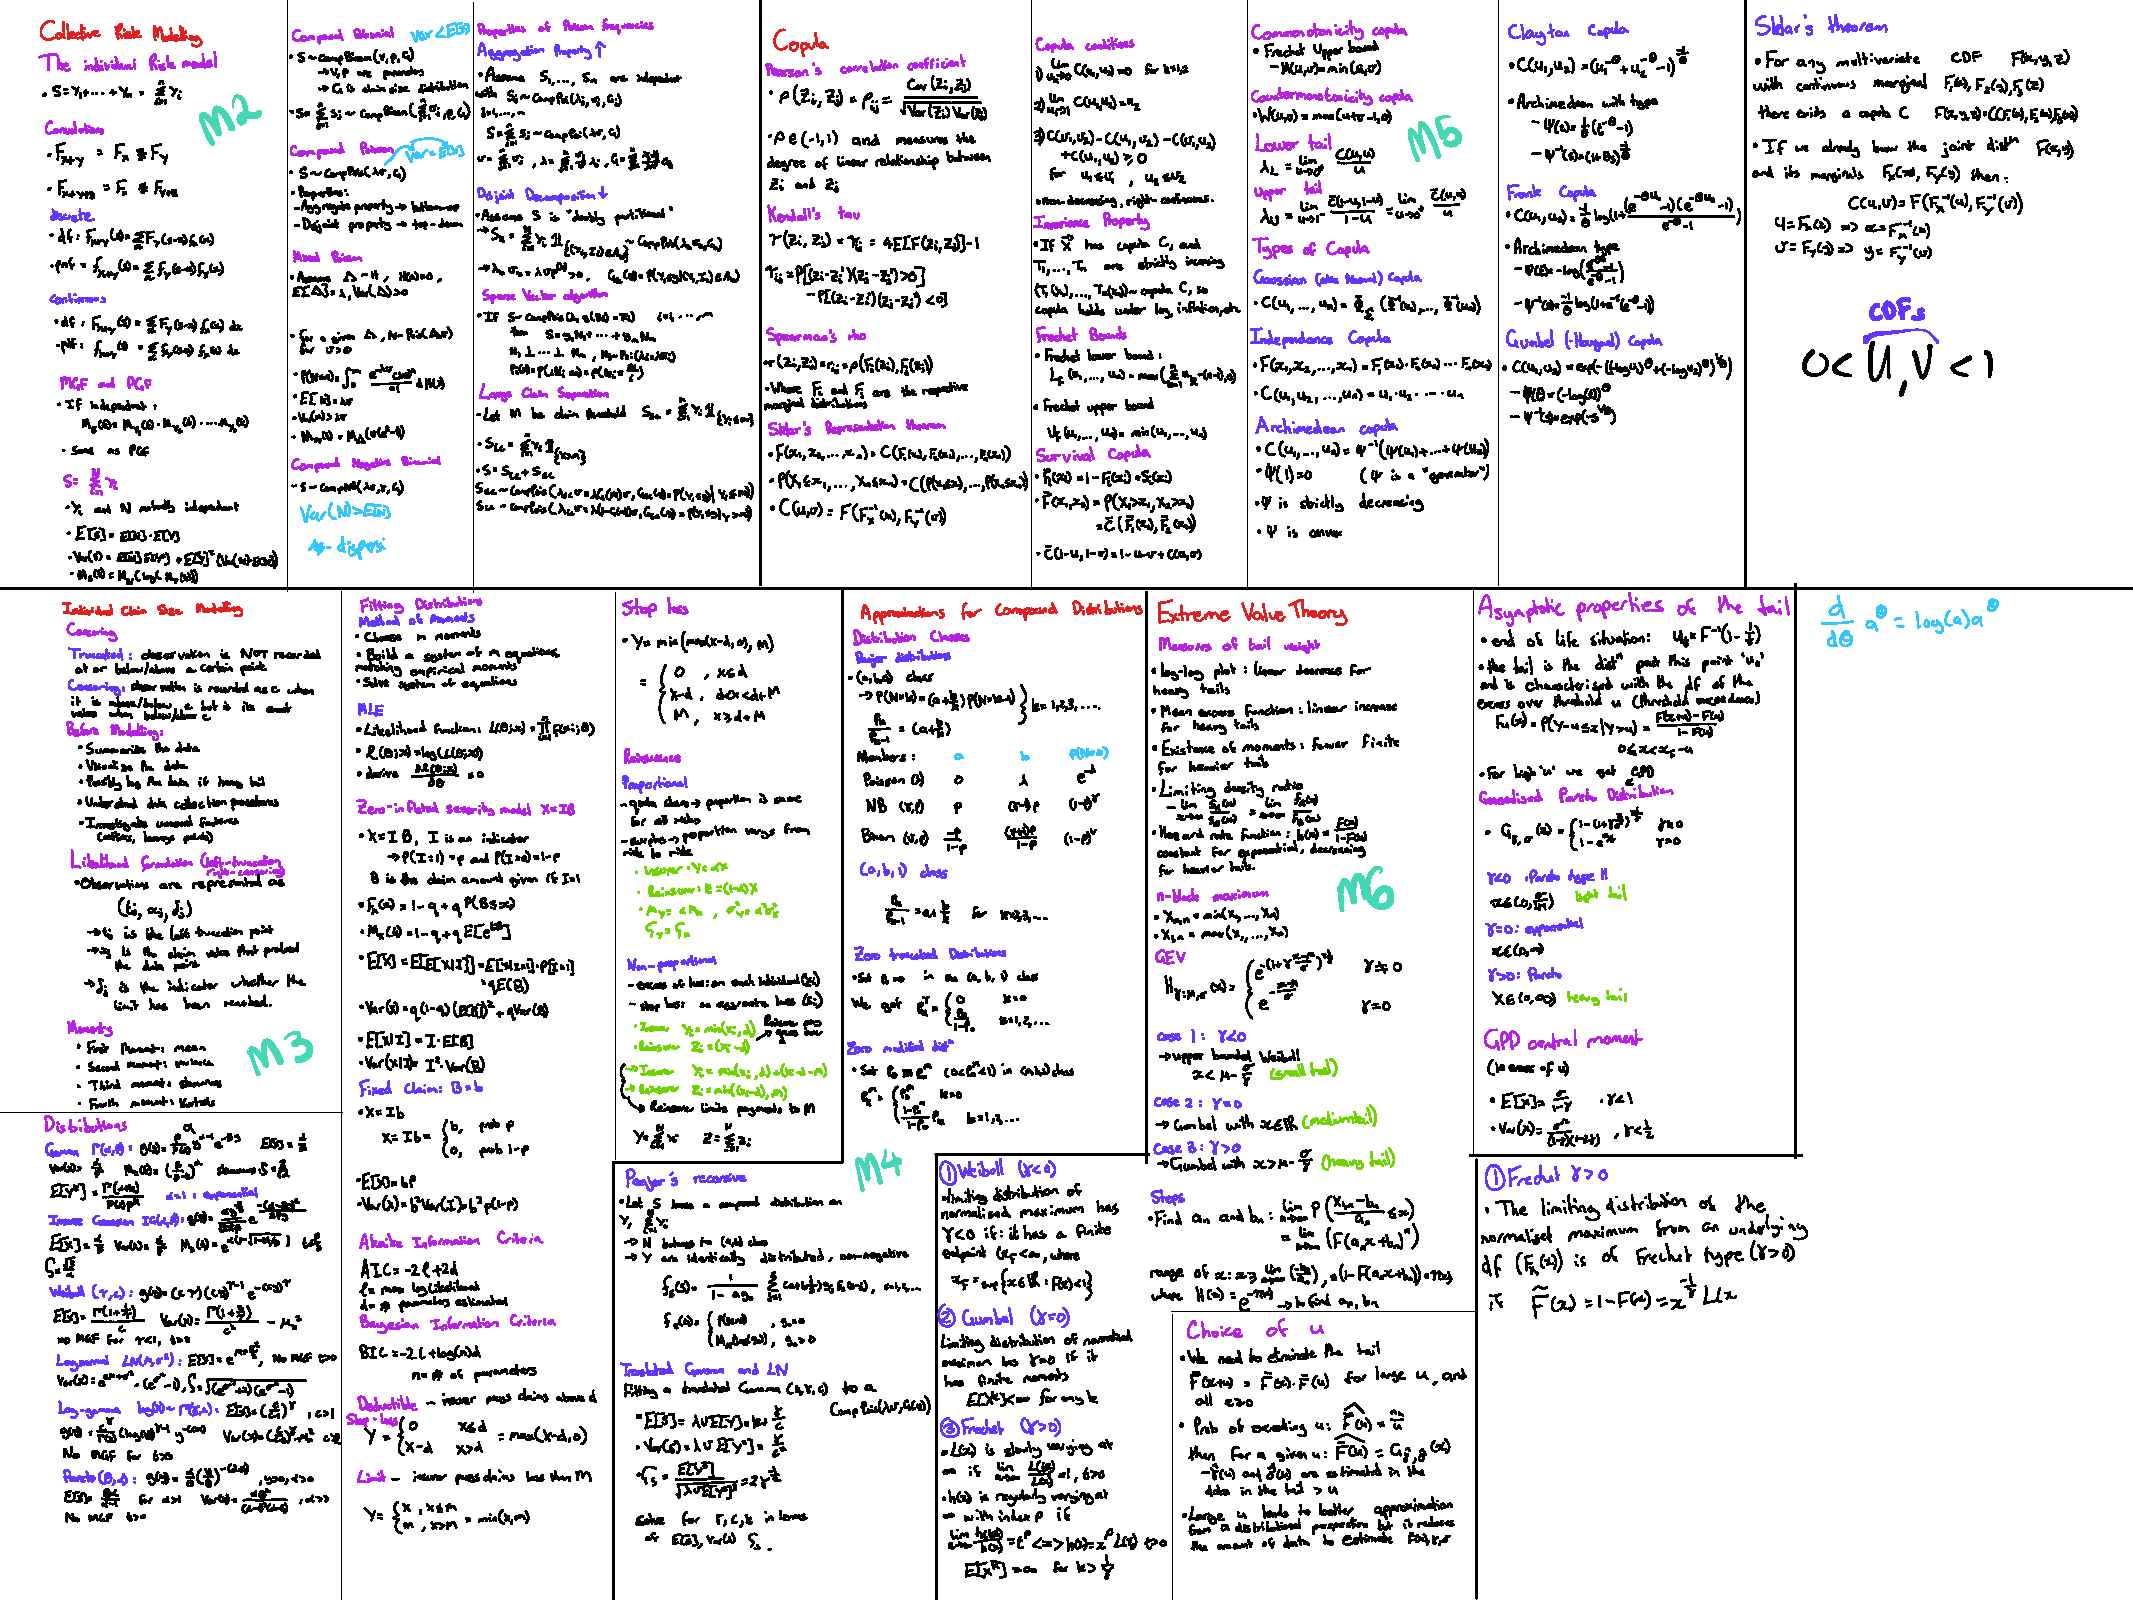
\includepdf[pages=-]{formula sheet (2).pdf}


\end{document}

